\documentclass{article}

% Submission: main track, double-blind.
% For camera-ready: \usepackage[main,final]{neurips_2026}
\usepackage{neurips_2026}

\usepackage[utf8]{inputenc}
\usepackage[T1]{fontenc}
\usepackage{hyperref}
\usepackage{url}
\usepackage{booktabs}
\usepackage{amsfonts}
\usepackage{nicefrac}
\usepackage{microtype}
\usepackage{xcolor}
\usepackage{amsmath,amssymb,amsthm}
\usepackage{graphicx}
\usepackage{bbm}
\usepackage{booktabs} % For \toprule, \midrule, \bottomrule
\usepackage{graphicx} % For \includegraphics
\usepackage{caption}  % For \captionof

% ------------------------------------------------------------------
%  Theorem environments  (single counter throughout)
% ------------------------------------------------------------------
\newtheorem{theorem}{Theorem}[section]
\newtheorem{proposition}[theorem]{Proposition}
\newtheorem{corollary}[theorem]{Corollary}
\newtheorem{lemma}[theorem]{Lemma}
\newtheorem{definition}[theorem]{Definition}
\newtheorem{remark}[theorem]{Remark}


\usepackage{todonotes}
% ------------------------------------------------------------------
%  Visible TODO markers (red, appear in compiled PDF)
% ------------------------------------------------------------------
\newcommand{\vtodo}[1]{%
  {\color{red}\textbf{[TODO:} \textit{#1}\textbf{]}}%
}

\newcommand{\note}{\textcolor{blue}}


% ------------------------------------------------------------------
%  Notation shorthands
% ------------------------------------------------------------------
\newcommand{\R}{\mathbb{R}}
\newcommand{\normF}[1]{\|#1\|_F}
\newcommand{\Ptgt}{P_{\mathrm{tgt}}}
\newcommand{\vecop}{\mathrm{vec}}

% ------------------------------------------------------------------
\title{Operator Projection for Depth-Robust Optimization in Factored Networks}

% Double-blind submission: no author information.
\author{Anonymous Author(s)}

\begin{document}
\maketitle

\begin{abstract}
Parameter-space optimization can be a poor proxy for function-space optimization in deep factored networks. We study this gap through the composed operator $P = W_L \cdots W_1$ and show that standard gradient updates of the factors do not realize the operator gradient step: each layer contributes a spectral distortion, producing a depth-dependent mismatch between the intended and actual motion of $P$. We propose to correct this mismatch directly via an operator-projection objective, which searches for factor updates whose product best matches a target operator-space update. In deep linear networks, this objective admits an Alternating Least Squares (ALS) solver with an explicit modewise form; this view also reveals K-FAC as a separable approximation to the operator-projection update. Since random initialization can independently cause spectral collapse of the context operators, we introduce a warm-start that preserves their singular values and makes the ALS sub-problems well conditioned. Across controlled linear, fixed-gate, and non-linear experiments, ALS with warm-start achieves accurate operator alignment and remains stable at depths where standard parameter-space optimizers collapse. These results support operator projection as a principled framework for diagnosing and correcting depth-induced optimization mismatch in factored networks.
\end{abstract}

% ==================================================================
\section{Introduction}
\label{sec:intro}
% ==================================================================
Modern deep networks are trained by updating weight parameters
$\{W_\ell\}$, yet their input-output behavior is governed by the composed
operator $P = W_L \cdots W_1$. This creates a mismatch between the space in
which optimization is performed and the space in which the model function is
realized. Existing work characterizes the dynamics and implicit bias of such
factorized models~\cite{saxe2014exact, gunasekar2017implicit}, while
natural-gradient methods address curvature in parameter space
\cite{martens2020new}. Our focus is complementary: we ask
whether a weight-space update actually realizes the operator-space step it is
intended to approximate.
%
The answer is already negative in the two-factor case $P = W_2 W_1$. Let $G$
be the gradient of the loss with respect to $P$. A direct operator-space
gradient step would move $P$ along $-\eta G$, whereas gradient descent on the
factors induces
\begin{equation*}
  \Delta P_{\mathrm{GD}}
  =
  -\eta(W_2 W_2^\top G + G W_1^\top W_1)
  + \eta^2 G W_1^\top W_2^\top G .
  \label{eq:gd-mismatch-intro}
\end{equation*}
Thus, even at first order, the operator update is a spectrally filtered version
of the desired operator step. At depth $L$, analogous context matrices surround
each layer update, so the mismatch can accumulate across the factorization.
%
We address this mismatch by changing the optimization primitive. Instead of
accepting the operator motion implicitly induced by weight-space gradients, we
formulate an operator-projection objective: given a target operator
$P_{\mathrm{tgt}}$, find weight increments whose updated product best matches
that target. For deep linear networks, this objective yields closed-form
least-squares sub-problems and can be solved by Alternating Least Squares (ALS).
The resulting modewise update exposes how the singular values of the left and
right contexts control each operator-space direction. It also clarifies the
connection to K-FAC: in the deep-linear isotropic setting, K-FAC corresponds to
a separable approximation of the ALS modewise denominator. 
%\todo{I would add a connection to the sections (see sections~\ref{sec:kfac} and~\ref{sec:als})}. 
Figure~\ref{fig:2d-traj} gives a concrete illustration. In a controlled
two-dimensional deep linear problem, ALS-Exact closely tracks the target
operator-space trajectory at both $L=2$ and $L=32$. By contrast, the tested
gradient-based baselines increasingly deviate as depth grows; in the deeper
case, K-FAC becomes unstable and exits the displayed frame. This example is
diagnostic rather than a benchmark: it visualizes the depth-induced operator
mismatch that motivates the operator-projection framework.

A separate obstacle is spectral collapse. Under standard random initialization,
products of random matrices can become increasingly anisotropic with depth: a
few directions dominate while many others are attenuated
\cite{haas2026jacobian, pennington2018emergence}. In this regime, the context
matrices that determine how layer updates affect the full product are poorly
conditioned. We therefore pair operator projection with a warm-start designed to
preserve the singular values of these contexts, so that the projection step can
act on the relevant operator directions. 

\begin{figure}[t]
  \centering
  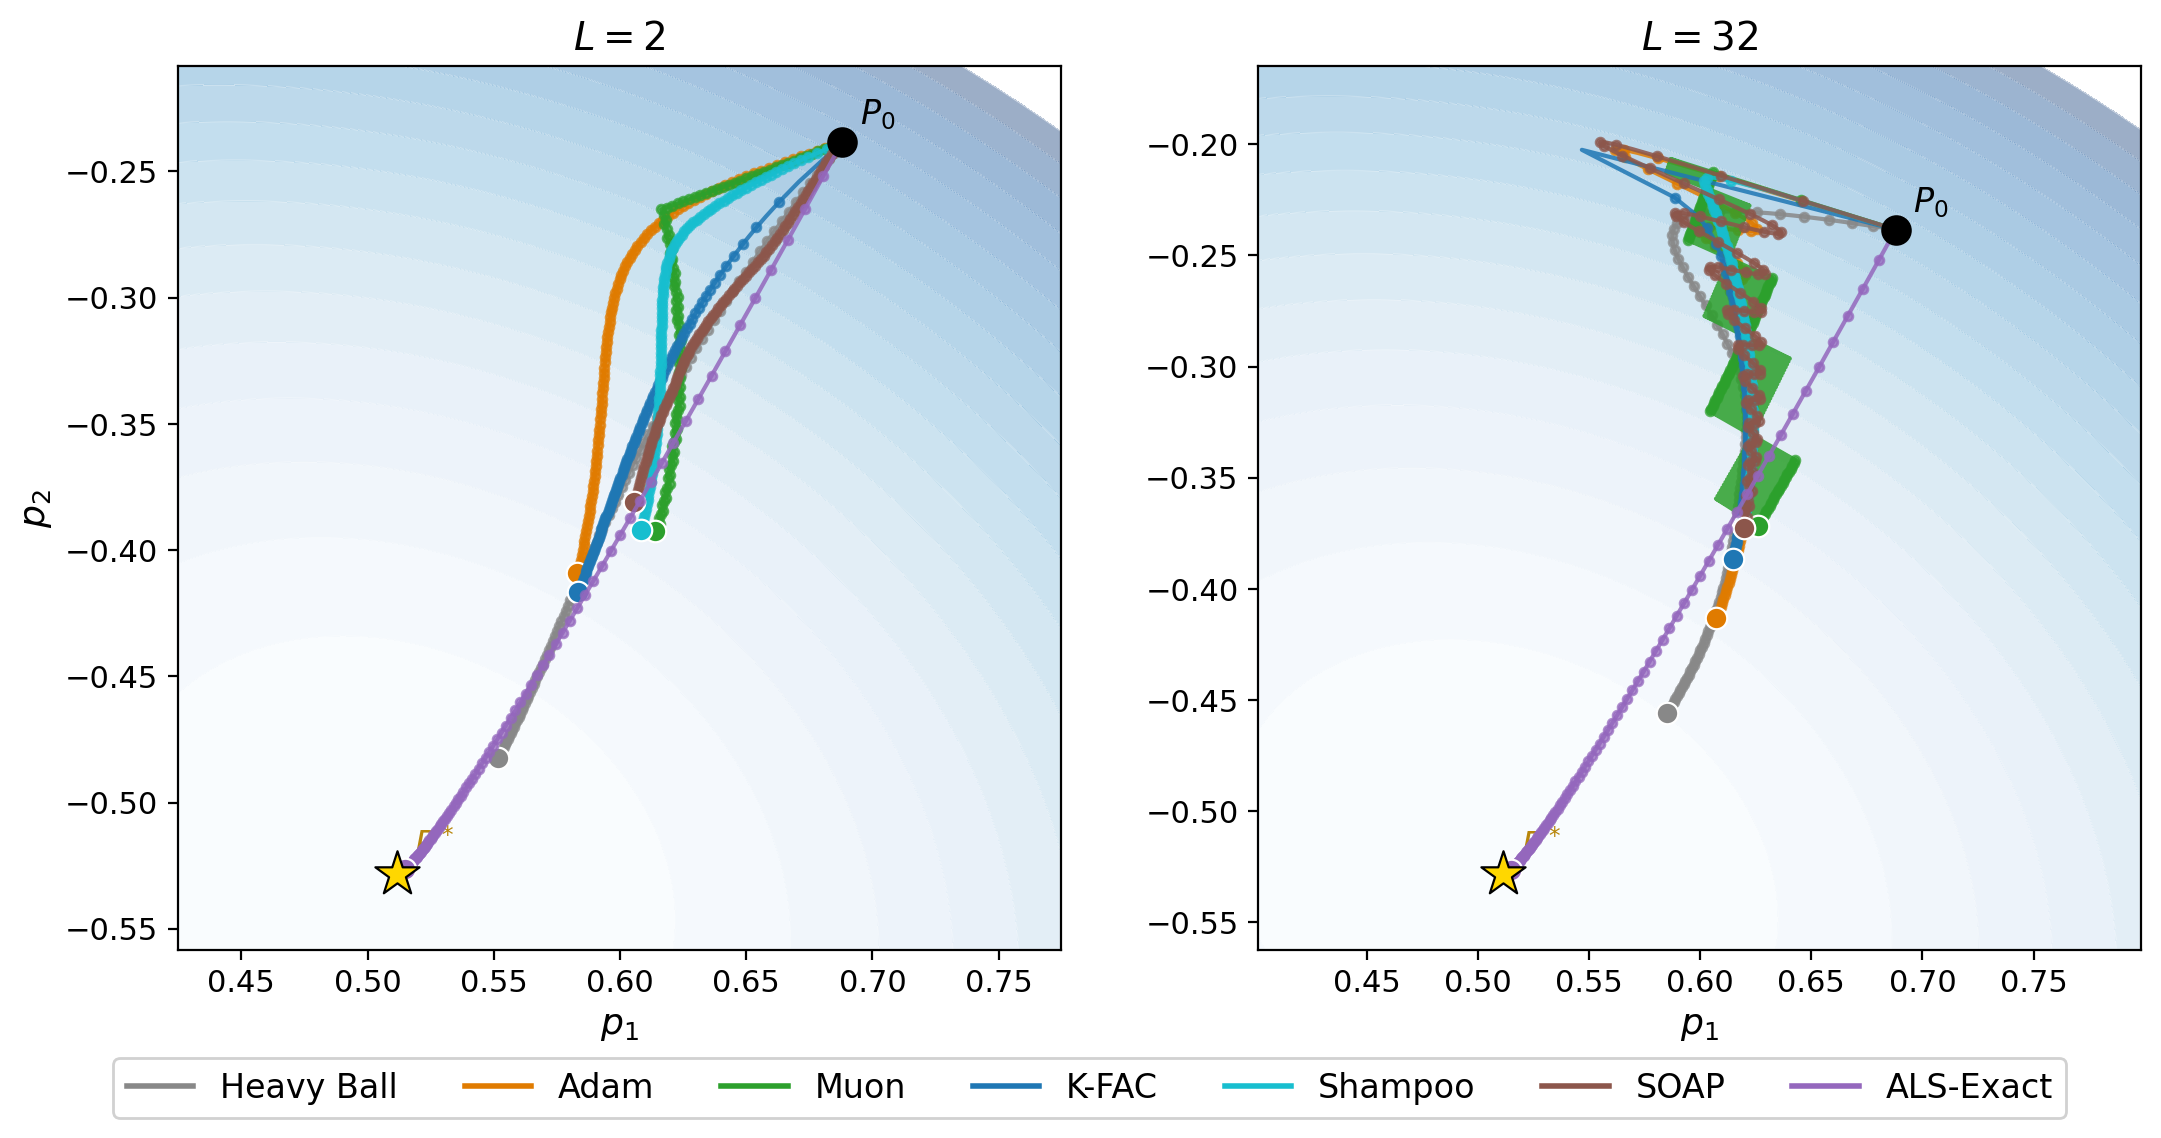
\includegraphics[width=0.6\linewidth]{images/toy_2d_trajectories.png}
  \caption{Diagnostic operator-space trajectories for deep linear networks of
  depths $L = 2$ (left) and $L = 32$ (right), using the same initial composed
  operator $P_0$. ALS-Exact closely tracks the target trajectory at both depths,
  whereas the tested gradient-based baselines increasingly deviate as depth
  grows. In the deeper case, K-FAC becomes unstable and exits the displayed
  frame.}
  \label{fig:2d-traj}
\end{figure}

Overall, our contribution is an operator-projection framework for diagnosing
and correcting depth-induced mismatch in factored networks. We identify the
spectral distortion induced by weight-space gradient updates, derive an ALS
solver for the corresponding projection problem in deep linear networks, relate
its modewise update to K-FAC, and show that warm-start initializations mitigate
the separate conditioning obstacle caused by spectral collapse. Across
controlled linear, fixed-gate, and non-linear experiments, ALS with warm-start
maintains operator alignment and remains stable in depth regimes where the
tested parameter-space baselines become ineffective.

% ==================================================================
\section{Related Work}
\label{sec:related}
% ==================================================================


\textbf{Deep linear networks and spectral collapse.}
Deep linear networks are a canonical testbed for studying optimization
geometry. Exact singular-value dynamics under gradient flow were derived by
\citet{saxe2014exact}, while subsequent work studied depth-induced implicit
acceleration, auto-balancing, and implicit regularization in matrix
factorization
\citep{arora2018optimization,du2018algorithmic,
gunasekar2017implicit,arora2019implicit}. These works analyze the operator
motion implicitly induced by parameter-space gradient descent. Our work changes
the primitive: we directly target a desired operator displacement and solve for
factor updates that realize it as closely as possible. A related spectral issue
is collapse at initialization, where products of random matrices become highly
anisotropic with depth~\citep{haas2026jacobian}. Our warm-start is motivated by
this phenomenon and aims to keep the context operators used by the ALS solver
well conditioned.

\textbf{Natural gradient, K-FAC, and matrix preconditioners.}
Natural-gradient methods precondition parameter updates using the Fisher metric
\citep{amari1998natural,martens2020new}. For deep linear networks,
\citet{bernacchia2018exact} derived exact natural-gradient updates with
Kronecker structure. K-FAC approximates Fisher blocks by Kronecker products of
activation and gradient covariances~\citep{martens2015optimizing}, with
extensions to convolutional and modern architectures
\citep{grosse2016kronecker,george2018ekfac,eschenhagen2023kfac}. Our objective
is different: it measures error in Frobenius norm on the composed operator,
rather than in a Fisher metric on parameter or distribution space. Nevertheless,
in the isotropic deep-linear setting, K-FAC can be viewed as a separable
approximation to the ALS modewise denominator; the exact comparison is given in section ~\ref{sec:kfac}. 
Shampoo and SOAP use accumulated gradient
statistics and matrix preconditioners rather than current context geometry
\citep{gupta2018shampoo,vyas2024soap}, with scalable implementations in
\citet{anil2021scalable,morwani2024shampoo}. We therefore treat them as
important empirical comparators, but not as algebraic approximations of the
operator-projection objective.

\textbf{Adaptive, spectral, and initialization methods.}
Adam and AdamW provide elementwise adaptivity through moving averages of
gradient moments~\citep{kingma2015adam,loshchilov2019decoupled}. Muon instead
orthogonalizes matrix gradients through Newton--Schulz iterations and is
closely related to matrix-sign or spectral-gradient methods
\citep{jordan2024muon,bernstein2024modular,kosson2024spectral,
kim2026muon,newtonmuon2026,liu2025muon}. These methods reshape or normalize
parameter-space gradients. Operator projection is complementary: it starts from
a desired end-to-end operator displacement and maps it back to factor updates.
Initialization has also been studied through signal propagation and dynamical
isometry
\citep{schoenholz2017deep,pennington2017resurrecting,pennington2018emergence}.
Our warm-start targets the conditioning of the per-layer context matrices
$A_k^\top A_k$ and $B_k B_k^\top$, which determine the ALS projection
sub-problems.

\textbf{Factorized training and low-rank adaptation.}
Optimization through factors appears in Burer--Monteiro parameterizations,
matrix factorization, and low-rank adaptation
\citep{burer2003nonlinear,hu2022lora,zhao2024galore,hayou2024lora}.
Initialization strategies for factorized layers have also been studied
\citep{khodak2021factorized}. These methods use factorization for structure,
parameter efficiency, or adaptation. Our work instead studies how factorization
distorts operator motion and derives updates that directly control the
represented operator.

% ==================================================================
\section{Operator Level Optimization}
\label{sec:framework}
% ==================================================================


%We structure the development of the operator-projection framework in progressive stages of architectural complexity. To isolate the fundamental optimization geometry from the compounding effects of non-linearities, Sections~\ref{sec:setup} and~\ref{sec:als} establish the gradient mismatch problem and our exact Alternating Least Squares (ALS) solver in the unconstrained setting of deep linear networks. Section~\ref{sec:kfac} grounds this exact mathematical solution in the existing literature, demonstrating that K-FAC emerges naturally as a specific, isotropic approximation of the ALS update. Finally, Section~\ref{sec:extensions} scales the framework to practical non-linear architectures (ReLU MLPs) via the frozen-gate linearization.

We develop the operator-projection framework in stages. Sections~\ref{sec:setup}
and~\ref{sec:als} isolate the basic geometry in deep linear networks, where the
composed operator is explicit and the layerwise projection sub-problems admit
closed-form solutions. Section~\ref{sec:kfac} relates the resulting modewise
update to K-FAC in the isotropic deep-linear setting. Section~\ref{sec:extensions}
then extends the formulation to fixed-gate linear networks and to ReLU MLPs
under frozen gates.

\subsection{Setup and the mismatch at depth}
\label{sec:setup}

For depth $L$, write $P = W_L \cdots W_1 \in \R^{n_L \times n_0}$ for the
composed operator and $G = \nabla_P \mathcal{L}(P) \in \R^{n_L \times n_0}$
for the operator-space gradient.
A natural choice of target is the steepest-descent step in operator space.
\begin{equation}
  \Ptgt = P - \eta G.
  \label{eq:operator-target}
\end{equation}

% {\color{red}The line above seems overly complicated to me. Why not simply write "The gradient update with respect to $W$ reads"
% \begin{align}
% W' = W - \eta G_W
% \end{align}
% and keep the notation $G_W$ for the operator gradient throughout?
% }


Consider the context matrices
% \begin{equation}
%   A_k = W_L \cdots W_{k+1} \in \R^{n_L \times n_k},
%   \qquad
%   B_k = W_{k-1} \cdots W_1 \in \R^{n_{k-1} \times n_0},
%   \label{eq:contexts-def}
% \end{equation}
  $A_k = W_L \cdots W_{k+1} \in \R^{n_L \times n_k}$ and 
$ B_k = W_{k-1} \cdots W_1 \in \R^{n_{k-1} \times n_0}$,
with $A_L = I_{n_L}$ and $B_1 = I_{n_0}$, so that $P = A_k W_k B_k$ for
each $k$.
The gradient descent updates $\Delta W_k = -\eta A_k^\top G B_k^\top$
induce an operator increment that, to first order in $\eta$, satisfies Proposition \ref{prop:gd-mismatch-deep}. 

\begin{proposition}[GD mismatch at depth $L$]
\label{prop:gd-mismatch-deep}
Under gradient descent with updates $\Delta W_k = -\eta A_k^\top G B_k^\top$
for $k = 1, \dots, L$, the induced operator increment is, to first order in
$\eta$,
\begin{equation}
  \Delta P_{\mathrm{GD}}
  = -\eta \sum_{k=1}^{L} A_k A_k^\top\, G\, B_k^\top B_k,
  \label{eq:gd-mismatch-deep}
\end{equation}
which is generically different from the desired $-\eta G$.
The distortion is a sum of left-right preconditioning terms, one per layer,
each weighted by the Gram matrices of corresponding context pair.
\end{proposition}
\begin{proof}
The exact operator increment under simultaneous updates $\{\Delta W_k\}$ is
$\Delta P = \sum_k A_k \Delta W_k B_k + O(\eta^2)$ to first order.
Substituting $\Delta W_k = -\eta A_k^\top G B_k^\top$ gives~\eqref{eq:gd-mismatch-deep}.
\end{proof}

For all possible operator gradients $G$, agreement with $-\eta G$ would require
$\sum_k A_k A_k^\top G B_k^\top B_k = G$ for all $G$, which imposes
$\sum_k A_k A_k^\top \otimes B_k^\top B_k = I$: a condition that is not
preserved along training trajectories.
The two-factor case from the introduction is the $L = 2$ instance of
Proposition~\ref{prop:gd-mismatch-deep}, with the single distortion term
$W_2 W_2^\top G + G W_1^\top W_1$.
At depth $L$, every layer contributes a context-dependent distortion term, so
the mismatch can accumulate with the number of factors.

\subsection{Operator-projection objective and ALS solver}
\label{sec:als}

The mismatch in Proposition~\ref{prop:gd-mismatch-deep} motivates replacing
the implicit operator motion induced by weight-space gradient descent with a
direct optimization of the operator displacement.
Given $\Ptgt$ from~\eqref{eq:operator-target}, we seek weight increments
$\{\Delta W_\ell\}$ whose updated product matches $\Ptgt$ as closely as
possible:
\begin{equation}
  \min_{\{\Delta W_\ell\}}
  \left\|
    \prod_{\ell=L}^{1}(W_\ell + \Delta W_\ell) - \Ptgt
  \right\|_F^2
  + \lambda \sum_{\ell=1}^{L} \normF{\Delta W_\ell}^2.
  \label{eq:eopp}
\end{equation}
This is non-linear in the $\Delta W_\ell$ jointly.
We solve it by Alternating Least Squares (ALS): at each sweep $t$ we iteratively update $\Delta W_\ell^{(t)}$. We visit layers in sequence and, for layer $k$, consider all $\ell \ne k$ at their current values. The contexts at iteration $t$ are $A_k^{(t)} = \prod_{\ell=L}^{k+1}(W_\ell + \Delta W_\ell^{(t)})$, $B_k^{(t)} = \prod_{\ell=k-1}^{1}(W_\ell + \Delta W_\ell^{(t)})$ and residual
$R_k^{(t)} = \Ptgt - A_k^{(t)} W_k B_k^{(t)}$, the layer-$k$ sub-problem is
\begin{equation}
  \min_{\Delta W_k}
  \normF{A_k^{(t)} \Delta W_k B_k^{(t)} - R_k^{(t)}}^2 + \lambda \normF{\Delta W_k}^2.
  \label{eq:als-sub}
\end{equation}
This is a standard Tikhonov-regularized least-squares problem in $\Delta W_k$.
For $\lambda>0$, the sub-problem is strongly convex in $\Delta W_k$ and has a
unique minimizer even when $A_k$ or $B_k$ is rank deficient.
The first-order optimality condition is the  equation
\begin{equation}
  (A_k^\top A_k)\, \Delta W_k\, (B_k B_k^\top) + \lambda \Delta W_k
  = A_k^\top R_k B_k^\top.
  \label{eq:stein}
\end{equation}
Let $A_k = U_A \Sigma_A V_A^\top$ and $B_k = U_B \Sigma_B V_B^\top$ be
compact SVDs, and set
$\widetilde{\Delta W}_k = V_A^\top \Delta W_k U_B$,
$\widetilde G_k = V_A^\top (A_k^\top R_k B_k^\top) U_B$. Since the right-hand side lies in the row and column spaces of the contexts and $\lambda>0$ penalizes null-space components, the minimizer has no component outside these subspaces.
Equation~\eqref{eq:stein} then decouples entry-wise:
\begin{equation}
  \widetilde{\Delta W}_{k,ij}
  = \frac{\widetilde G_{k,ij}}{\sigma_{A,i}^2\, \sigma_{B,j}^2 + \lambda},
  \label{eq:modewise}
\end{equation}
with $\Delta W_k = V_A \widetilde{\Delta W}_k U_B^\top$.
Each mode of the projected gradient $\widetilde G_k$ is filtered by the product
of the corresponding context singular values: 
Modes with large context singular values require smaller weight increments to produce a given operator displacement, whereas directions with small context singular values are dominated by the regularizer and are difficult to correct.
The cost is $O(n_k^3 + n_{k-1}^3)$ per layer per sweep via the two compact SVDs.
We use reverse Gauss--Seidel sweep order $k = L, \dots, 1$ throughout, which seemed
empirically better for stability and convergence speed.
% \todo{mention where the empirical claim is supported}

\subsection{Relation to K-FAC}
\label{sec:kfac}
Under the standard K-FAC factorization, the layer k update is
% \begin{equation}
%   \Delta W_k^{\mathrm{KFAC}}
%   = -\eta\, \hat G_\lambda^{-1}\, G_{W_k}\, \hat A_\lambda^{-1},
%   \label{eq:kfac-update}
% \end{equation}
$  \Delta W_k^{\mathrm{KFAC}}
  = -\eta\, \hat G_\lambda^{-1}\, G_{W_k}\, \hat A_\lambda^{-1}$,
where $G_{W_k} = \nabla_{W_k}\mathcal{L}$ is the weight gradient,
% \textcolor{red}{Is it $G_{W_k} = A_k^\intercal G B_k^\intercal$ or is it $G_{W_k} = A_k^\intercal R_k B_k^\intercal$ where $R_k$ is the residual used above? If it is $G_{W_k} = A_k^\intercal G B_k^\intercal$ then you need to be careful because the $\tilde{G}$ are not the same. They are close though but if I'm not mistaken they are not exactly the same. I think it is fine but you need to write $R_k$ since you work with $\Delta W_k$}
% \note{No this is not the same problem as my ALS solve, there is absolutely no $R_k$ there, in KFAC we just use the fisher matrix as a curvature correction of the weight gradient, no residual anywhere this is specific to ALS}
$\hat A = \mathbb{E}[hh^\top]$ is the input activation covariance,
$\hat G = \mathbb{E}[\delta\delta^\top]$ is the pre-activation gradient
covariance, and $\hat A_\lambda = \hat A + \lambda I$,
$\hat G_\lambda = \hat G + \lambda I$.
In the deep linear factorization $P = A_k W_k B_k$ we have,
$G_{W_k} = A_k^\top G B_k^\top$, $G = \nabla_ P \mathcal{L}$.
With $h = B_k x$ and $\delta = A_k^\top g$ with $g$ the output gradient signal, we have $\hat A = B_k \Sigma_x B_k^\top$ and
$\hat G = A_k^\top \Sigma_g A_k$, where $\Sigma_x = \mathbb{E}[xx^\top]$ and
$\Sigma_g = \mathbb{E}[g g^\top]$.
% \textcolor{red}{Check my note but I think that the pre-activation gradient is given by $A_k^\intercal Px$ and not $A_k^\intercal Pxx^\intercal = A_k^\intercal \nabla_P \mathcal{L}$. Fro this reason, I'm not sure that requiring isotropy of $\nabla_P \mathcal{L}$ is enough. I believe you need isotropy of $Pxx^\intercal$ and I'm not sure it is equivalent. Do you take the expectation with respect to $P$ or $x$? It depends on the assumptions you make on $P$ and $x$ I think. Now because the expectation is taken with respect to the input data distribution in the definition of the Fisher matrix, you can just require $x\|x\|$ to be isotropic. This works for Gaussian inputs I think.}
When the input distribution is isotropic ($\Sigma_x = I$) and the gradient
distribution is isotropic ($\Sigma_g = I$), these reduce to
$\hat A = B_k B_k^\top$ and $\hat G = A_k^\top A_k$, so the K-FAC
diagonalization basis is exactly $(V_A, U_B)$:  the same basis as the ALS
modewise solution~\eqref{eq:modewise}.
In this basis, the K-FAC modewise update is
\begin{equation}
  \widetilde{\Delta W}_{k,ij}^{\mathrm{KFAC}}
  = \frac{\widetilde G_{k,ij}}{(\sigma_{A,i}^2 + \lambda)(\sigma_{B,j}^2 + \lambda)},
\end{equation}
versus the ALS denominator $\sigma_{A,i}^2 \sigma_{B,j}^2 + \lambda$. Using the same scalar damping parameter $\lambda$ for comparison, the gap between the two is
\begin{equation}
  (\sigma_{A,i}^2 + \lambda)(\sigma_{B,j}^2 + \lambda)
  - (\sigma_{A,i}^2 \sigma_{B,j}^2 + \lambda)
  = \lambda(\sigma_{A,i}^2 + \sigma_{B,j}^2 + \lambda - 1),
  \label{eq:kfac-gap}
\end{equation}
which is non-zero in general and grows with $\lambda$.
K-FAC can therefore be understood as solving the operator-projection
sub-problem~\eqref{eq:als-sub} with an approximate denominator, valid
when the data distribution is approximately isotropic.
Outside this assumption the K-FAC diagonalization basis differs from
$(V_A, U_B)$ and the comparison is no longer exact.

\begin{remark}
Shampoo and SOAP are derived from accumulated gradient outer products rather
than current context geometry, and their diagonalization bases coincide with
$(V_A, U_B)$ only when both context matrices are approximate isometries.
Adam ignores the left-right Kronecker structure entirely.
We include all three as empirical comparators without claiming an algebraic
connection to the operator-projection objective.
\end{remark}

\subsection{Extension to gated and non-linear networks}
\label{sec:extensions}

\textbf{Fixed-gates linear networks.}
Following~\cite{haas2026jacobian}, the Jacobian of a piecewise-linear network along a fixed activation pattern is a product of weight matrices interleaved with fixed diagonal gate matrices. 
%This is called a Fixed-Gates Linear Network
%(FGLN):
\begin{equation}
  P = W_L D_{L-1} W_{L-1} \cdots D_1 W_1,
  \label{eq:fgln}
\end{equation}
where each $D_\ell \in \R^{n_\ell \times n_\ell}$ is a fixed diagonal matrix.
The ALS sub-problem~\eqref{eq:als-sub} has the same form as the deep linear case, the only change is that the contexts now absorb the gate factors. $A_k = W_L D_{L-1} \cdots W_{k+1} D_k$, and 
  $B_k = D_{k-1} W_{k-1} \cdots D_1 W_1$. The mode-wise solve~\eqref{eq:modewise} then applies without modification.


\textbf{ReLU MLPs.}
For a ReLU MLP without bias terms, the output for sample $x_b$ under the frozen-gate linearization is governed by the sample-specific linear operator
\begin{equation}
  P(x_b) = W_L D_{L-1}(x_b) \cdots D_1(x_b) W_1,
  \label{eq:mlp-operator}
\end{equation}
where $D_\ell(x_b) = \mathrm{diag}(\mathbbm{1}[z_\ell(x_b) > 0])$ is the
ReLU gate at layer $\ell$. We use the convention $D_0 = D_L = I$.
This makes each sample's operator a FGLN with sample-specific gates,
and the MLP is a multi-mode FGLN where the gate pattern is determined by the
input.
%
Let $\delta_b = \partial \mathcal{L} / \partial \hat y_b \in \R^{n_L}$ be the
output gradient for sample $b$ and $x_b \in \R^{n_0}$ the network input.
Under the frozen-gate linearization, the operator-space gradient at sample $b$
is the rank-one matrix $\delta_b x_b^\top$, and the per-sample operator target
is
% \begin{equation}
%   \Ptgt(x_b) = P(x_b) - \eta\, \delta_b x_b^\top.
%   \label{eq:mlp-target}
% \end{equation}
  $\Ptgt(x_b) = P(x_b) - \eta\, \delta_b x_b^\top$.
Averaging over a batch of $B$ samples with frozen gates, the batched
operator-projection objective is
\begin{equation}
  \min_{\{\Delta W_\ell\}}
  \frac{1}{B} \sum_{b=1}^B
  \left\| \prod_{\ell=L}^1 D_\ell(x_b) (W_\ell + \Delta W_\ell) - \Ptgt(x_b) \right\|_F^2
  + \lambda \sum_\ell \normF{\Delta W_\ell}^2.
  \label{eq:mlp-objective}
\end{equation}

For layer $k$ and sweep iteration $t$, with per-sample contexts $A_k(x_b)^{(t)}$, $B_k(x_b)^{(t)}$ defined as
in~\eqref{eq:fgln} with sample-specific gates and current $\Delta W_\ell^{(t)}$ values, and residuals
$R_{k,b}^{(t)} = \Ptgt(x_b) - A_k(x_b)^{(t)}\bar W_k B_k(x_b)^{(t)}$, the ALS layer-$k$
sub-problem at iteration $t$ is
\begin{equation}
  \min_{\Delta W_k}
  \frac{1}{B}\sum_{b=1}^B
  \normF{A_k(x_b)^{(t)}\,\Delta W_k\,B_k(x_b)^{(t)} - R_{k,b}^{(t)}}^2
  + \lambda \normF{\Delta W_k}^2,
  \label{eq:mlp-als-sub}
\end{equation}
The exact normal equation for~\eqref{eq:mlp-als-sub} is obtained by
vectorizing and differentiating, giving
\begin{align}
  \left(
    \frac{1}{B}\sum_{b=1}^B B_k(x_b)^{(t)}B_k(x_b)^{(t)\top} \otimes A_k(x_b)^{(t)\top} A_k(x_b)^{(t)}
    + \lambda I
  \right) \vecop(\Delta W_k) \nonumber
  \\= \vecop\!\left(\frac{1}{B}\sum_{b=1}^B A_k(x_b)^{(t)\top} R_{k,b}^{(t)} B_k(x_b)^{(t)\top}\right).
  \label{eq:mlp-exact-normal}
\end{align}
The system matrix is a \emph{sum} of Kronecker products, one per sample,
and does not factor as a single Kronecker product in general.
It therefore cannot be diagonalized via a joint SVD, and solving it directly
costs $O(n_k^3 n_{k-1}^3)$ per layer. We call this \emph{ALS-exact}.
%
\emph{ALS-MN} replaces the sum of Kronecker products by the Kronecker product
of the batch-averaged Gram matrices:
\begin{equation}
  \frac{1}{B}\sum_{b=1}^B B_k(x_b)B_k(x_b)^\top \otimes A_k(x_b)^\top A_k(x_b)
  \;\approx\;
  N_k \otimes M_k,
  \label{eq:mn-approx}
\end{equation}
where $M_k = \frac{1}{B}\sum_b A_k(x_b)^\top A_k(x_b)$ and
$N_k = \frac{1}{B}\sum_b B_k(x_b)B_k(x_b)^\top$.
This approximation treats the per-sample context Gram matrices as independent
of each other across the batch, which is equivalent to assuming that
$A_k(x_b)^\top A_k(x_b)$ and $B_k(x_b)B_k(x_b)^\top$ do not co-vary across
samples.
Under this approximation the normal equation becomes
\begin{equation}
  M_k\, \Delta W_k\, N_k + \lambda\, \Delta W_k
  = \frac{1}{B}\sum_{b=1}^B A_k(x_b)^\top R_{k,b} B_k(x_b)^\top,
  \label{eq:mlp-mn-normal}
\end{equation}
which has the same  structure as~\eqref{eq:stein} and is solved by the
modewise formula~\eqref{eq:modewise} with $M_k$ and $N_k$ in place of
$A_k^\top A_k$ and $B_k B_k^\top$, at cost $O(n_k^3 + n_{k-1}^3)$.
The approximation~\eqref{eq:mn-approx} becomes exact when $B = 1$, and
improves as the per-sample Gram matrices concentrate around their batch means.
Table \ref{tab:cost} reports all costs. Further variants are described in Appendix~\ref{app:variants}.









%%%%%%%%%%%%%%%%%%%%%%%%%%%%%%%%%%%%%%%%%%%%%%%%%%%%%%%%%%%%%%%%%%%%%%%%%%%%%%%%%%%%%%%%%%%%%%%%%%%%%%%%%%%%%%%%%%%%%%%%%%%%%%%%%%%%%%%%%%%
\section{Spectral collapse and warm-start initialization}
\label{sec:warm-start}
The ALS solver requires the context matrices $A_k$, $B_k$ to be
sufficiently well-conditioned for the modewise
solution~\eqref{eq:modewise} to produce meaningful operator corrections.
Under standard random initialization at depth $L$, this condition is not met.
The singular values of products of random matrices separate exponentially with
depth~\cite{haas2026jacobian}: a few dominant modes grow while the rest
collapse toward zero.
In the collapsed regime, $\sigma_{A,i}^2 \sigma_{B,j}^2 \ll \lambda$ for
nearly all mode pairs $(i,j)$, and the modewise solution reduces to
$\widetilde{\Delta W}_{k,ij} \approx \widetilde G_{k,ij} / \lambda$: a
uniform rescaling of the gradient with no operator-correcting structure.
This mirrors the conditioning mechanism behind vanishing-gradient behavior in
deep products, but here it appears directly in the ALS contexts.
%
We therefore use a warm-start that moves the working factors to a well-conditioned reference before the first projection step. The goal is to make the relevant context singular values non-degenerate, up to rank constraints imposed by gates.

\textbf{Deep linear.}
For square layers, initialize the unkown $\Delta W_\ell^{(0)}$ so the full operator is the identity:
\begin{equation}
  \Delta W_\ell^{(0)} = I_{n_\ell} - W_\ell, \qquad \ell = 1, \dots, L.
  \label{eq:warm-start-linear}
\end{equation}
For this initialization $P = I$ and all context singular values equal $1$, so
every gradient mode is correctable equally.

\begin{remark}
  With $\lambda = 0$, after the warm-start all working weights equal $I$ and
  all context matrices are identity.
  The first ALS sweep, starting at layer $L$, then reduces to
  $\min_{\Delta W_L^{(1)}} \|\Delta W_L^{(1)} - (\Ptgt - I)\|_F^2$,
  giving $\Delta W_L^{(1)} = \Ptgt - I$ with zero residual.
  All other layers receive zero additional increments.
  The non-trivial regime is $\lambda > 0$, where the regularization in
  \eqref{eq:eopp} prevents any single layer from absorbing the full update
  and forces the operator correction to be distributed across all $L$ layers
  according to the projection objective.
  The identity warm-start for deep linear networks is essentially an artefact needed to avoid spectral collapse; the algorithmic content
  of the operator-projection objective is most visible in the FGLN and MLP
  settings below.
\end{remark}

\textbf{FGLN.}
With fixed diagonal masks $D_\ell$, define active index sets
$\mathcal{I}_{\ell-1} = \{j : (D_{\ell-1})_{jj} = 1\}$ and
$\mathcal{I}_\ell = \{i : (D_\ell)_{ii} = 1\}$.
For each layer $\ell$, construct an orthogonal matrix $O_\ell$ that routes
the $r_\ell = \min(|\mathcal{I}_{\ell-1}|, |\mathcal{I}_\ell|)$ active
input coordinates to active output coordinates, completing the inactive
complement to a full orthogonal map via any orthogonal extension.
Initialize $\Delta W_\ell^{(0)} = O_\ell - W_\ell$.
After this update, the end-to-end operator $P$ has an isometric singular
profile up to the rank permitted by the gates: all non-zero singular values
equal $1$.
This is the core case where the warm-start is genuinely non-trivial, since
the gate structure makes a uniform identity initialization impossible and the
orthogonal routing construction is tailored to the network's active subspace
geometry.

% \textcolor{red}{If you have some time. The last part of the above paragraph is not very clear to me. From what you say it seems you can just initialize the $\Delta W$ to $I$ so I don't understand why you say that the warm-start is not trivial. It cannot be uniformly equal to the identity because of the gates that I get.}
% \note{No I say exactly that you cannot initialize to identity since the gates would still make things collapse. And we never initialize $\Delta W_\ell$ as identity, but as $I -W_\ell $ in deep linear case. So indeed $W_\ell + \Delta W_\ell$ would be identity. But now multiply by the gates, the previous gate and next gates zeroes out some rows and columns, so if the two gates zeroes out disjoint rows and columns we end up with the zero matrix, we have to specifically tailor the initialization so that the layer maps the active space of the previous gate to the active space of the next one. How would you reformulate above ? What part is not clear ?}

% {\color{red} Do you initialize $\Delta W$ or $\Delta (D_{\ell}WD_{\ell-1})$ ? My point is if you don't initialize the gates, you cannot prevent the vanishing initialization (for $P$) to happen right?}

% \note{I initialize only $\Delta W$, and yes that's the point we can still prevent the collapse completely through orthogonal initialization well tailored to the active gates (through permutation in fact, we just prmute the active ones so that they match across layers in some way).}

% {\color{red} OK. I think I see, you will have smaller non zero blocks if the supports are disjoints but the gates select the rows and columns so you might still have a non zero matrix}



\textbf{MLP.}
For a batch of inputs $\{x_b\}_{b=1}^B$ with frozen activation gates
$\{D_\ell(x_b)\}$, compute per-sample orthogonal maps $O_{\ell,b}$ by the
FGLN construction applied to each sample's gate pattern, and initialize
\begin{equation}
  \Delta W_\ell^{(0)} = \frac{1}{B}\sum_{b=1}^B O_{\ell,b} - W_\ell.
  \label{eq:warm-start-mlp}
\end{equation}
This is the mean of per-sample orthogonal mappings and is not itself
orthogonal in general; it is a heuristic that averages the active-subspace
alignment across the batch.
It is empirically effective in our experiments but does not carry a formal
conditioning guarantee, and may fail at extreme depths, large batches or unusual activation geometries.


% \begin{figure}[t]
%   \centering
%   % --- Left Side: The Table ---
%   \begin{minipage}{0.48\textwidth}
%     \centering
%     \captionof{table}{One-step alignment in the 2D toy setting
%       ($L = 2$, $h = 2$, $N = 100$, $\lambda = 10^{-4}$, Xavier init).
%       Cosine is measured between $\Delta P$ and the ideal operator direction
%       $P^\star - P_0$, normalized.}
%     \label{tab:2d-cos}
%     \scriptsize
%     \begin{tabular}{lcc}
%       \toprule
%       Method     & Cosine w.r.t.\ $\Delta P^\star$ & $\Vert \Delta P \Vert_F$ \\
%       \midrule
%       Heavy Ball & 0.90  & $8.2 \times 10^{-4}$ \\
%       Adam       & 0.72  & $4.5 \times 10^{-3}$ \\
%       Muon       & 0.72  & $2.6 \times 10^{-3}$ \\
%       K-FAC      & 0.97  & $5.2 \times 10^{-2}$ \\
%       Shampoo    & 0.72  & $8.1 \times 10^{-3}$ \\
%       SOAP       & 0.63  & $3.0 \times 10^{-3}$ \\
%       ALS-Exact  & 1.00  & $7.9 \times 10^{-3}$ \\
%       \bottomrule
%     \end{tabular}
%   \end{minipage}
%   \hfill % This adds spacing between the two minipages
%   % --- Right Side: The Figure ---
%   \begin{minipage}{0.48\textwidth}
%     \centering
%     \caption{One-step update directions in operator space ($L = 2$, $h = 2$,
%       Gaussian init). Each arrow shows $\Delta P = P_\mathrm{new} - P_0$
%       normalized to equal length.}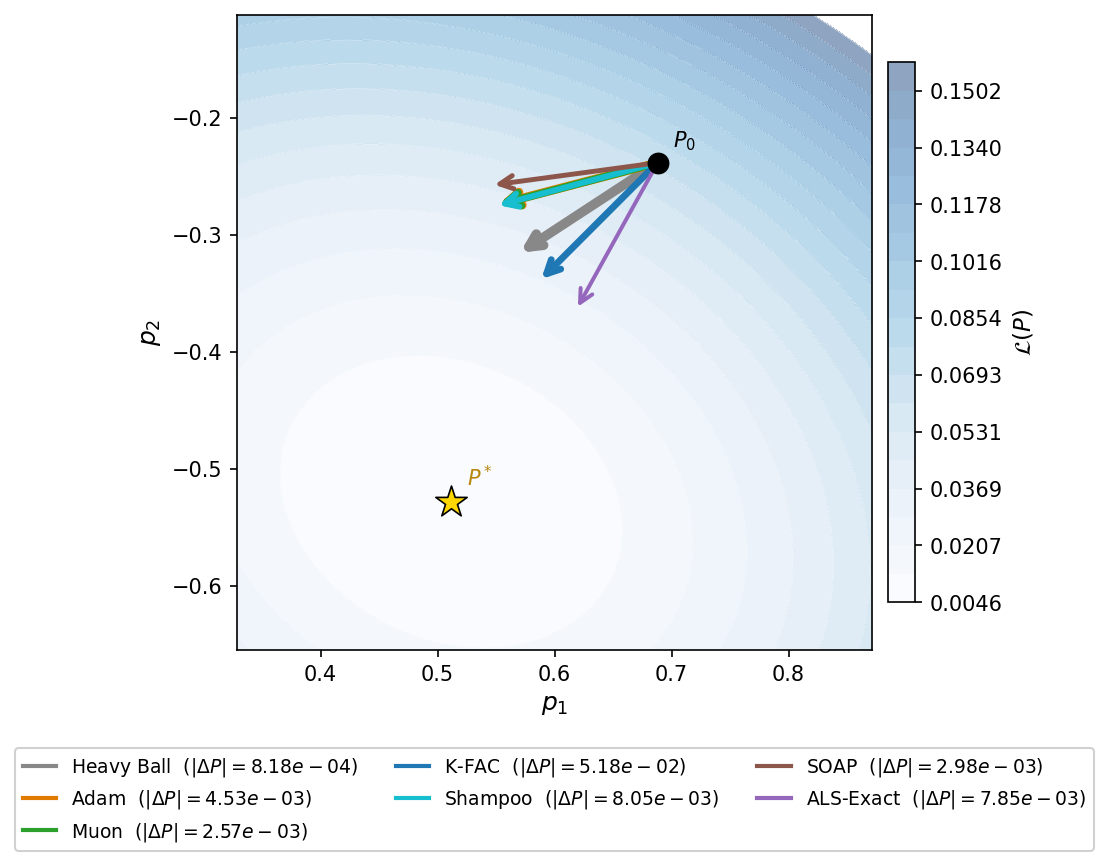
\includegraphics[width=\linewidth]{images/toy_2d_L2_h2.png}
%     \label{fig:2d}
%   \end{minipage}
% \end{figure}

\begin{table}[t]
  \centering
  \caption{One-step alignment in the 2D toy setting
    ($L = 2$, $h = 2$, $N = 100$, $\lambda = 10^{-4}$, Xavier init).
    Cosine is measured between $\Delta P$ and the ideal operator direction
    $P^\star - P_0$, normalized.}
  \label{tab:2d-cos}
  \scriptsize
  \begin{tabular}{lcc}
    \toprule
    Method     & Cosine w.r.t.\ $\Delta P^\star$ & $\Vert \Delta P \Vert_F$ \\
    \midrule
    Heavy Ball & 0.90  & $8.2 \times 10^{-4}$ \\
    Adam       & 0.72  & $4.5 \times 10^{-3}$ \\
    Muon       & 0.72  & $2.6 \times 10^{-3}$ \\
    K-FAC      & 0.97  & $5.2 \times 10^{-2}$ \\
    Shampoo    & 0.72  & $8.1 \times 10^{-3}$ \\
    SOAP       & 0.63  & $3.0 \times 10^{-3}$ \\
    ALS-Exact  & 1.00  & $7.9 \times 10^{-3}$ \\
    \bottomrule
  \end{tabular}
\end{table}





\begin{figure}[t]
  \centering
    \caption{Convergence to $P^\star$ under Xavier initialization ($d = 16$,
    $L = 128$, $N = 64$, isotropic target, up to $10{,}000$ steps).
    ALS-exact is early-stopped at step $677$ having reached $2 \times 10^{-10}$;
    all gradient-based baselines remain at initialization-level error
    (${\approx}0.97$) under spectral collapse.}
  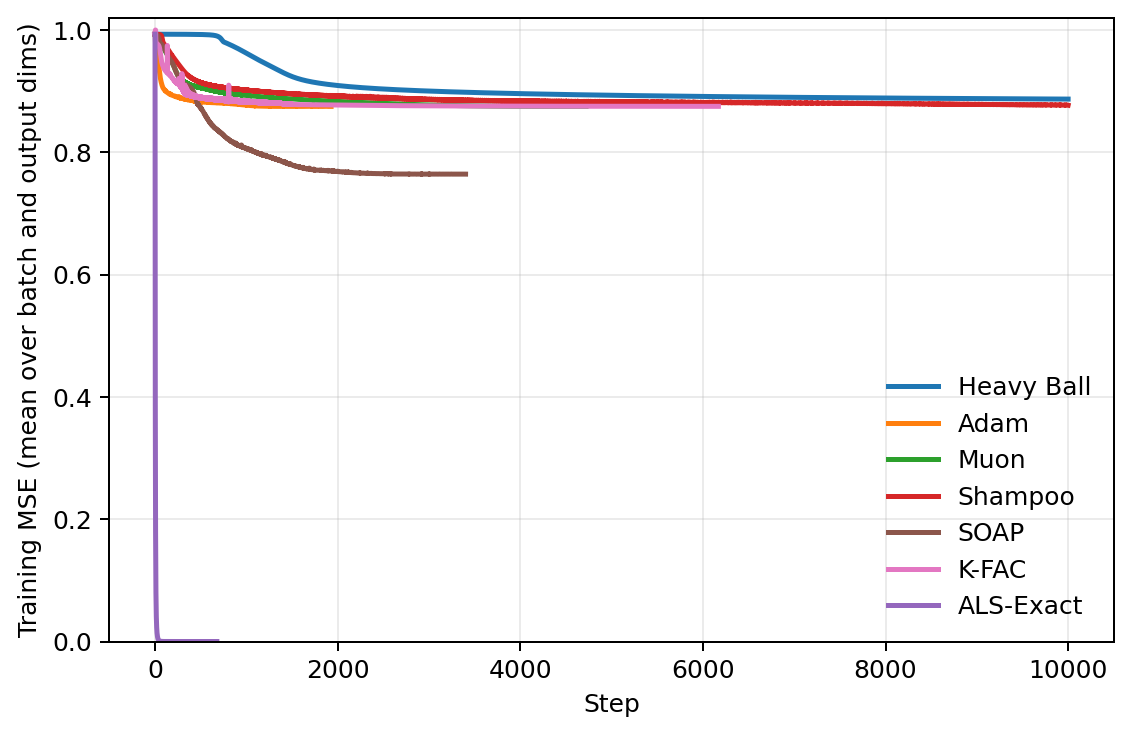
\includegraphics[width=0.4\linewidth]{images/deeplinear_convergence.png}
  \label{fig:deeplinear-convergence}
\end{figure}


% ==================================================================
\section{Experiments}
\label{sec:experiments}
% ==================================================================

We evaluate our methods across three experimental environments of increasing complexity\footnote{All experiments have been done on a single GPU (Nvidia RTX 6000 Ada). Code is available anonymously at \url{https://anonymous.4open.science/r/Operator-Level-optimization-B0E8/README.md}
}: a 2D synthetic regression task (Section~\ref{sec:exp-2d}), deep linear and FGLN under simulated targets (Section~\ref{sec:exp-deeplinear}), and deep ReLU MLPs (Section~\ref{sec:exp-mlp}). Each of these subsections respectively presents experiments designed to address one of those three primary research questions: \emph{ (1) Local Alignment:} Does the operator-projection objective correctly resolve the one-step gradient mismatch compared to standard and preconditioned baselines? \emph{(2) Depth and Conditioning:} Can the framework successfully optimize deep linear and fixed-gate operators at depths where accumulated mismatch and spectral collapse defeat parameter-space methods? \emph{(3) Non-linear Scalability (proof-of-concept):} Does the frozen-gate approximation provide useful optimization behavior in deep ReLU MLPs?

\textbf{Synthetic Task Setup}
For our 2D and deep linear/FGLN experiments, we employ a synthetic teacher-student regression task. We define a target operator $P^\star$ and generate $N$ Gaussian input samples $x$, with labels given by $y = x^\top P^\star + \varepsilon$, where $\varepsilon \sim \mathcal{N}(0, 0.01)$. The student is a deep linear model $f(x) = W_L \cdots W_1 x$, and performance is measured by the relative operator error $\normF{P(t) - P^\star} / \normF{P^\star}$, where $P(t) = W_L(t) \cdots W_1(t)$.


\textbf{Baselines}
\label{sec:exp-protocol}
We compare ALS-exact against six parameter-space baselines: Heavy Ball (SGD with momentum), Adam~\cite{kingma2015adam}, Muon~\cite{jordan2024muon}, K-FAC~\cite{martens2015optimizing}, Shampoo~\cite{gupta2018shampoo}, and SOAP~\cite{vyas2024soap}.
%

\subsection{Operator-space geometry}
\label{sec:exp-2d}
To address local alignment, we use a 2D synthetic task with $n_0=2$, $n_L=1$, and $N=100$, so that $P^\star \in \mathbb{R}^{1\times 2}$ can be visualized directly in operator space. All methods start from the same Xavier initialization. ALS-exact uses learning rate $1.0$ with $\lambda=10^{-4}$, while baselines use learning rate $10^{-3}$. Figure~\ref{fig:2d} shows that ALS-exact follows the desired operator update exactly, whereas baseline directions are distorted. Figure~\ref{fig:2d-traj} shows that this local advantage compounds over training: ALS-exact rapidly approaches $P^\star$ for both $L=2$ and $L=32$, while baselines remain misaligned, with degradation increasing at depth. Table~\ref{tab:2d-cos} confirms perfect one-step alignment for ALS-exact ($\cos=1.00$); K-FAC is the closest gradient-based baseline ($\cos=0.97$), but still falls short. These results show that ALS-exact effectively optimizes in operator space, while parameter-space methods suffer from depth-amplified directional mismatch. We next test whether this local advantage translates into global convergence in deeper architectures.




\begin{figure}[t]
  \centering
  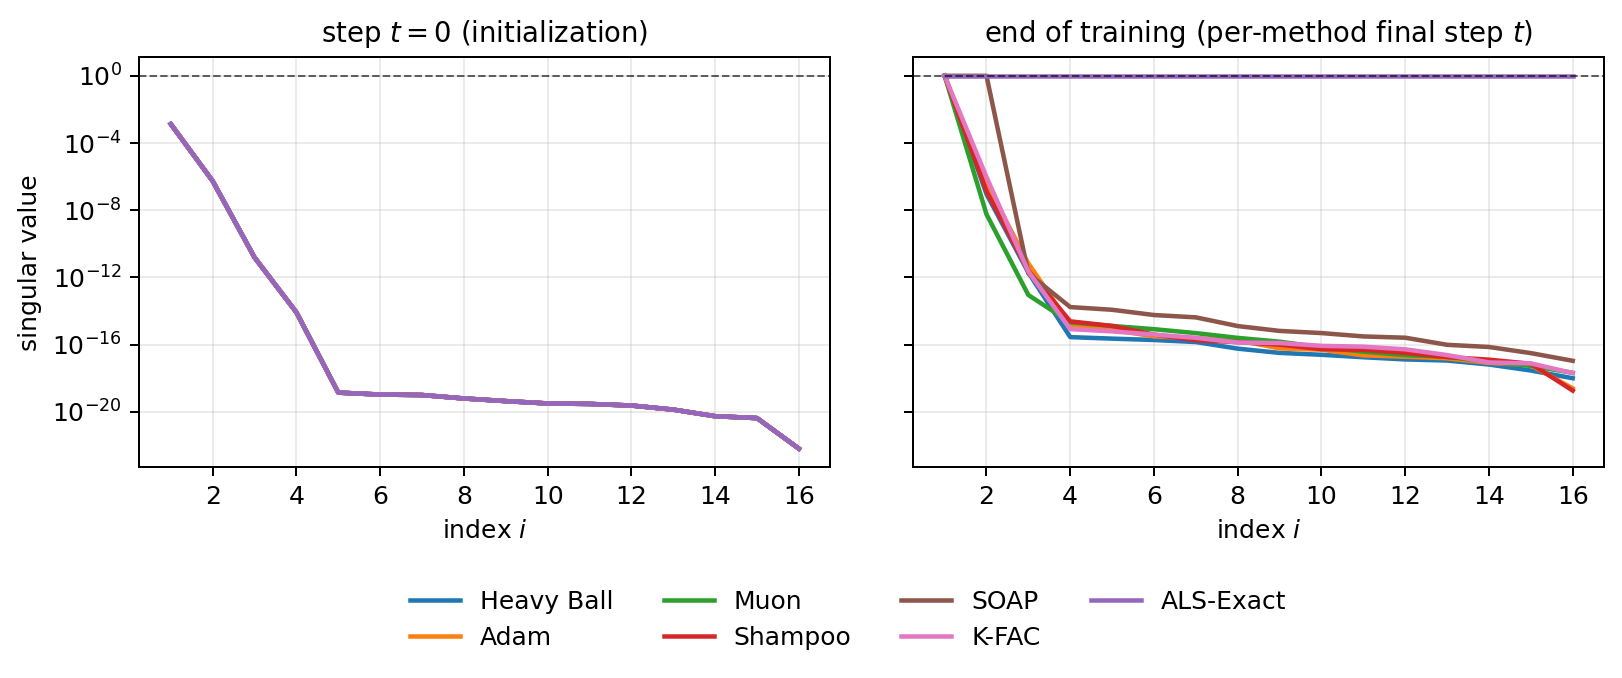
\includegraphics[width=0.65\linewidth]{images/deeplinear_spectrum.png}
  \caption{Singular-value spectrum of $P(t)$, Xavier initialization ($L = 128$).
    ALS-exact progressively matches the isotropic target; baselines remain
    compressed and recover only dominant modes.}
  \label{fig:deeplinear-spectrum}
\end{figure}
\begin{figure}[t]
  \centering
  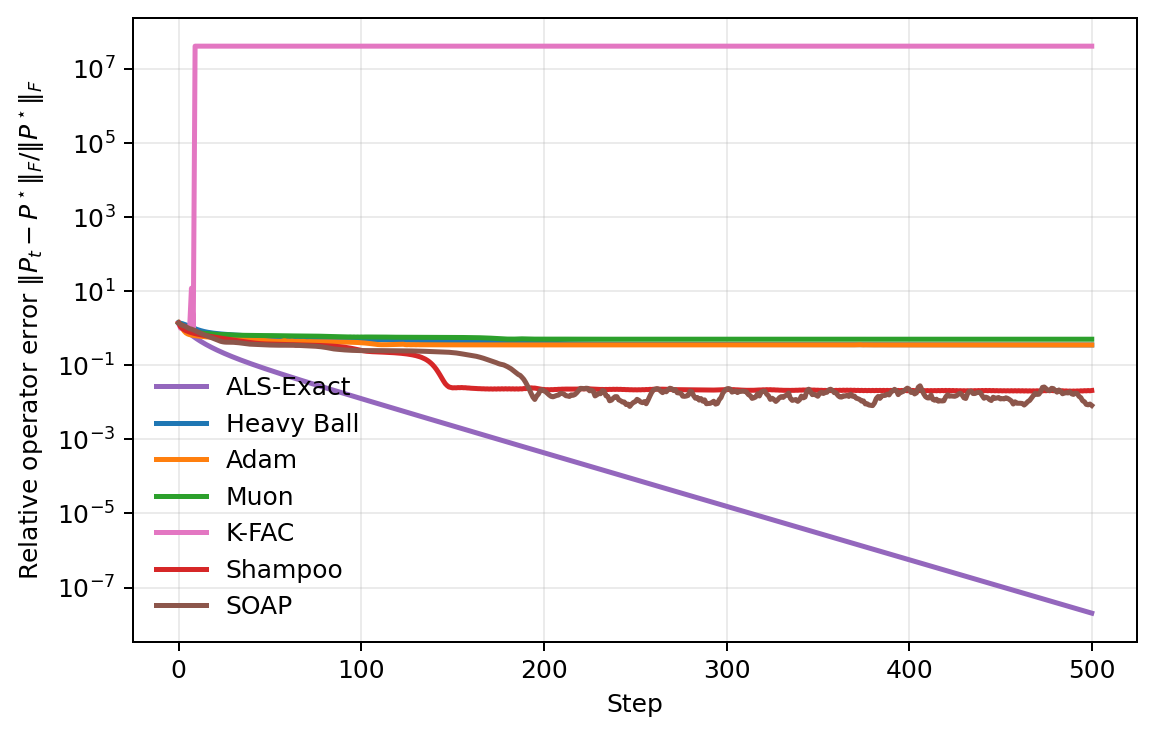
\includegraphics[width=0.39\linewidth]{images/deeplinear_convergence_identity.png}
  \caption{Convergence to $P^\star$ under identity initialization ($d = 16$,
    $L = 128$, $N = 64$, isotropic target, $500$ steps, $\lambda = 0$).
    All context singular values equal $1$ throughout, eliminating spectral
    collapse.  Despite perfect conditioning, gradient-based methods stall
    above $3.5 \times 10^{-1}$; ALS-exact reaches near machine precision
    (${\approx}2 \times 10^{-8}$), isolating  update-direction mismatch
    as  fundamental obstacle.}
  \label{fig:deeplinear-convergence-identity}
\end{figure}




\subsection{Deep linear and gated networks: recovery under depth and conditioning}
\label{sec:exp-deeplinear}
While the 2D case exposes the geometry, we next test whether the advantage scales to high-dimensional, very deep networks up to $L=128$. To separate update-direction mismatch from spectral collapse, we consider three initialization regimes. All experiments use hidden width $d=16$, $N=64$ samples, and an isotropic orthogonal target $P^\star$ in float64.

\textbf{Xavier initialization (ill-conditioned).}
Under Xavier initialization at $L=128$, context singular values separate exponentially and the operator spectrum collapses. Figure~\ref{fig:deeplinear-convergence} reports relative operator error over up to $10{,}000$ steps, with early stopping at $5\times10^{-5}$. Heavy Ball, Adam, Muon, Shampoo, SOAP, and K-FAC all stall near their initialization error ($\approx 0.97$), as spectral collapse destroys gradient information in most operator directions regardless of optimizer. In contrast, ALS-exact reaches $2\times10^{-10}$ by step $677$, near machine precision. This regime therefore confounds direction mismatch with vanishing gradients. Figure~\ref{fig:deeplinear-spectrum} confirms that gradient-based optimizers keep the spectrum collapsed, whereas ALS-exact with warm-start fully recovers it. Direct operator optimization thus succeeds in a regime where parameter-space optimizers fail.

\textbf{Identity initialization (well-conditioned).}
To isolate direction mismatch, we repeat the $L=128$ experiment with identity initialization ($W_k=I$, $\lambda=0$), removing spectral collapse since all context singular values equal $1$. Even then, Figure~\ref{fig:deeplinear-convergence-identity} shows that Heavy Ball, Adam, and Muon remain above $3.5\times10^{-1}$ after $500$ steps, while SOAP and Shampoo reach only $8\times10^{-3}$ and $2\times10^{-2}$. ALS-exact instead reaches $2\times10^{-8}$. Figure~\ref{fig:deeplinear-spectrum-identity} shows that ALS-exact recovers the flat target spectrum, whereas gradient-based methods become anisotropic. Thus, at depth $128$, direction mismatch, not conditioning, is the dominant obstruction.

\textbf{FGLN with warm-start (ill-conditioned gates).}
To test recovery under non-linear routing, we evaluate a depth-$128$ FGLN with fixed Bernoulli diagonal gates ($p=0.9$). These gates preclude uniform identity initialization and induce an ill-conditioned start. With our orthogonal warm-start, ALS-exact escapes the collapsed basin and recovers the target spectrum, whereas baselines fail to recover a conditioned geometry. See Appendix~\ref{app:exp-fgln}.

\begin{figure}[t]
  \centering
  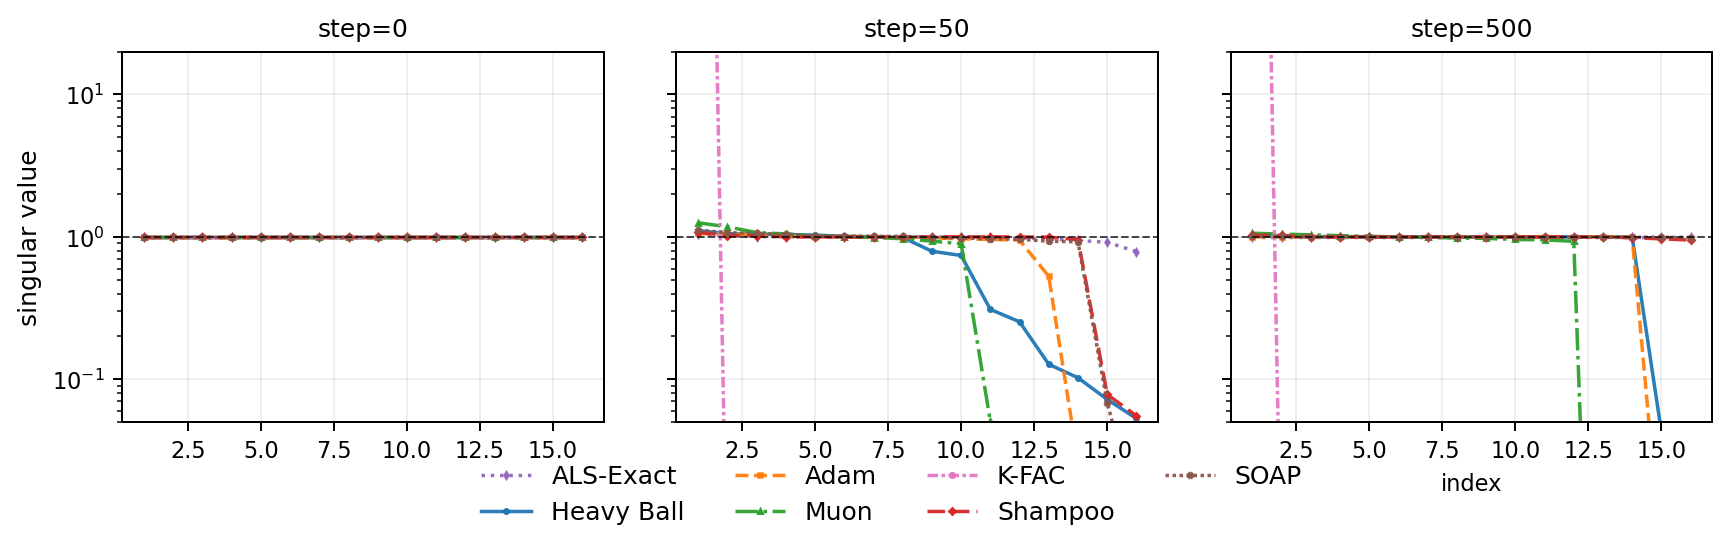
\includegraphics[width=0.85\linewidth]{images/deeplinear_spectrum_identity.png}
  \caption{Singular-value spectrum of $P(t)$ under identity initialization
    at steps $\{0, 50,500\}$.
    ALS-exact rapidly recovers the flat isotropic target spectrum.
    Gradient-based methods produce increasingly anisotropic operators
    even when starting from a perfectly conditioned initialization.}
  \label{fig:deeplinear-spectrum-identity}
\end{figure}
\begin{figure}[t]
  \centering
  \includegraphics[width=0.38\linewidth]{images/mnist_mlp_depth.png}
  \caption{MNIST depth sweep for bias-free MLPs $784\to[32]^L\to10$ with Xavier initialization. Each point reports the best validation loss over tested learning rates. ALS-exact ($\lambda=10^{-4}$, $10$ sweeps) remains trainable at $L=32$, where gradient-based baselines collapse to chance-level loss.}
  \label{fig:mnist-depth}
\end{figure}




\subsection{MLP depth scaling with frozen-gate local objective}
\label{sec:exp-mlp}
The previous experiments validated the framework for linear operators. We now test its extension to non-linear networks via the frozen-gate approximation. We train bias-free ReLU MLPs $784 \to [32]^L \to 10$ on MNIST for $L \in {1,2,4,8,16,32}$, using Xavier initialization, batch size $128$, and up to $50$ epochs with early stopping. The width $h=32$ keeps ALS-exact tractable while remaining sufficient for MNIST. We report the best validation loss over checkpoints and learning-rate sweeps.
ALS-exact uses learning rate $1.0$, $\lambda=10^{-4}$, and $10$ reverse sweeps per outer step, with ALS-MN used for the first large layer. Baselines sweep learning rates in ${10^{-2},10^{-3},10^{-4},10^{-5}}$, and results are averaged over $3$ seeds with variance bars. Figure~\ref{fig:mnist-depth} shows that ALS-exact performs best across depths and remains trainable at $L=32$, where all gradient-based baselines collapse. This supports the operator-mismatch analysis: increasing depth amplifies weight-space misalignment, while the frozen-gate ALS solve preserves alignment.


% ==================================================================
\section{Conclusion}
\label{sec:conclusion}
% ==================================================================

% We have studied operator-targeted optimization in deep factored networks from a
% theory-first perspective.
% The operator-projection objective is well-posed and depth-agnostic by
% construction, and ALS provides a principled solver whose block sub-problems are
% strongly convex and uniquely solvable under mild regularization.
% In deep linear and FGLN settings, ALS with warm-start achieves depth-invariant
% operator recovery up to $L = 32$, including regimes where all parameter-space
% methods fail entirely.
% In ReLU MLPs, a frozen-gate surrogate preserves trainability at $L = 32$ where
% standard baselines collapse.

% Several directions are open: extending the warm-start analysis to MLPs with
% formal guarantees; deriving tractable approximations to the exact MLP solve or extending the operator framework to other architectures. For example RNNs may benefit greatly from an operator perspective, where recursion induces strong depth and are known for their training instability. the current framework let freedom for the target oeprator update $\Delta P^*$, here we simply defined it as the gradient direction of the operator, but more sophisticated methods in the operator space could be helpfull.
% The warm-start strategy for $\Delta W_\ell$ may also be a research direction for a full network initialization strategy improving conditioning on the data for any kind of optimizers not limited to our ALS solver.
We studied operator-targeted optimization in deep factored networks. The operator-projection objective is well posed and depth-agnostic, and ALS gives a principled solver with strongly convex regularized block subproblems. In deep linear and FGLN settings, ALS with warm-start achieves depth-invariant recovery up to $L=32$, including regimes where parameter-space methods fail; in ReLU MLPs, a frozen-gate surrogate preserves trainability at the same depth. Future work includes extending the analysis to non-linear MLPs, approximating the exact MLP solve, applying the operator view to RNNs, designing richer operator-space updates beyond $\Delta P^\star$, and studying warm-start as a broader data-conditioned initialization strategy.

% ------------------------------------------------------------------
\begin{ack}
% Hidden in anonymous submission; fill in for camera-ready.
\end{ack}
% ------------------------------------------------------------------


\bibliographystyle{plainnat}
\bibliography{references}



% ==================================================================
%  APPENDIX  (unlimited pages, does not count toward page limit)
% ==================================================================
\newpage
\appendix


% ==================================================================
\section{Discussion and Limitations}
\label{sec:discussion}
% ==================================================================

\paragraph{Scope of claims.}
Our central claim is theoretical: the operator-projection
objective~\eqref{eq:eopp} and its MLP analogue~\eqref{eq:mlp-objective} are
well-posed, depth-agnostic by construction, and yield update directions better
aligned with the desired operator motion than parameter-space gradient descent.
We do not claim that ALS is a practical optimizer.
Its per-step cost --- $O(Ld^3)$ for deep linear/FGLN and $O(Ld^6)$ for the
exact MLP solve --- far exceeds the $O(Ld^2)$ cost of Adam or Muon.
The value of the current results is conceptual: they isolate depth-induced
mismatch as the explanatory variable and demonstrate that resolving it enables
learning in regimes where parameter-space methods cannot.

\textbf{Depth-agnostic objective vs.\ depth-agnostic solver.}
The \emph{objective} is depth-agnostic --- the minimizer of~\eqref{eq:eopp}
exists and is unique for all $L$ --- while the \emph{solver} is not
automatically so.
ALS inherits the same spectral collapse pathology as gradient-based methods
when context matrices have near-zero singular values: the modewise denominator
$\sigma_{A,i}^2 \sigma_{B,j}^2 + \lambda$ is dominated by $\lambda$, and
the solve loses its operator-correcting effect.
The warm-start of Section~\ref{sec:warm-start} moves the factor state away from
these degenerate basins before the first sweep.
For deep linear and FGLN this is provably effective: the identity/orthogonal
initialization yields well-conditioned contexts from which ALS proceeds to
near machine precision.
For MLPs the warm-start is empirically effective but lacks a formal guarantee;
establishing formal conditions under which it succeeds is an important open
problem.

\textbf{Frozen-gate approximation.}
The MLP extension freezes activation patterns within each outer step, treating
per-sample operators as fixed during the ALS sweep.
This is a first-order approximation analogous to Gauss--Newton linearization.
The approximation degrades when weight increments are large relative to
pre-activation margins; re-linearizing at each sweep is a principled but
costly alternative that we didn't experiment on.

\textbf{Experimental scope.}
The deep linear and FGLN experiments cleanly establish the theoretical claims.
The MNIST MLP experiments are narrow in scope (width $32$, no bias) and should not be read as general benchmarks.



\begin{table}[t]
\centering
\scriptsize
\caption{Per-step optimizer computational scaling in a square width $d$ network.}
\label{tab:cost}
\begin{tabular}{lll}
  \toprule
  Method                        & Cost per step  & Regime \\
  \midrule
  GD / Adam                     & $O(L d^2)$     & general \\
  Muon                          & $O(L d^3)$     & general \\
  ALS-exact (deep linear/FGLN)  & $O(L d^3)$     & exact \\
  ALS-MN (MLP)                  & $O(L d^3)$     & approximate \\
  ALS-exact (MLP)               & $O(L d^6)$     & proof-of-concept \\
  \bottomrule
\end{tabular}
\end{table}





\section{Solver Variants and Approximations}
\label{app:variants}

\subsection{Mean field approximation}
\label{app:mean-field}


For a generic batch objective
\[
\min_{\Delta \theta}\; \frac1B\sum_{b=1}^B \mathcal L_b(\Delta\theta),
\]
the exact minimizer is
\[
\Delta\theta^\star \in \arg\min_{\Delta\theta}\; \frac1B\sum_b \mathcal L_b(\Delta\theta).
\]
The per-sample-then-mean approximation computes
\[
\Delta\theta_b^\star \in \arg\min_{\Delta\theta}\; \mathcal L_b(\Delta\theta),
\qquad
\bar{\Delta\theta}=\frac1B\sum_b \Delta\theta_b^\star.
\]
In general,
\[
\arg\min_{\Delta\theta}\; \mathbb E_b[\mathcal L_b(\Delta\theta)]
\;\neq\;
\mathbb E_b\!\left[\arg\min_{\Delta\theta}\; \mathcal L_b(\Delta\theta)\right],
\]
so this is an expectation/minimization swap approximation.

In operator terms, the exact batched objective couples all samples through one
shared update $\Delta W_\ell$, whereas per-sample solves produce different
$\Delta W_{\ell,b}$ adapted to each sample's contexts and gates. Averaging these
solutions is only exact in special aligned regimes (e.g., identical contexts or
quadratic objectives with shared Hessian). Otherwise it introduces a bias that
can be large under gate heterogeneity.

This paradigm can be applied to any solver variants, so we present it here once
as a global approximation template.

In general we found that such an approximation was not accurate enough to get to the results exposed in this paper in the MLP case, and is trivially equivalent in the deep linear or FGLN case to the exact methods.

\subsection{Linearized operator objective: exact and block-diagonal variants}
\label{app:linobj}

Given current weights, contexts $A_\ell(x_b),B_\ell(x_b)$, and operator target
increment $\Delta P_b^\star$, the linearized objective is
\[
\min_{\{\Delta W_\ell\}}
\frac1B\sum_{b=1}^B
\left\|
\sum_{\ell=1}^L A_\ell(x_b)\,\Delta W_\ell\,B_\ell(x_b)-\Delta P_b^\star
\right\|_F^2
\;+\;
\lambda\sum_{\ell=1}^L \|\Delta W_\ell\|_F^2.
\]

\paragraph{Exact (coupled) solve.}
Vectorizing each layer update yields one coupled normal equation over all
layer blocks:
\[
\mathbf H\,\Delta \mathbf w = \mathbf g,
\]
where off-diagonal blocks $\mathbf H_{\ell m}$ encode cross-layer interactions
through shared sample contexts. This is the most faithful solve of the linearized
objective but is computationally expensive and memory-heavy at MLP scale. It is still however an approximation and less accurate than the exact ALS solver presented\todo{I would add "in section~\ref{app:dnc}"which exact solver? Also by linearized you mean that you only retain the first order approximation? Do you say "exact" because you do sweeps so that the increments remain small enough?}, which solved the real non-linear objective. The only difference in implementation to the ALS solver is that ALS takes into account the solves of each layer before solving the other layers\todo{This part is not clear. I thought the ALS solver was doing sweeps. I.e updating the weights sequentially}, while here we solve each layer once independently\todo{Do you mean that your ALS solver is an iterative solver while here you do a direct inversion?}, and it is equivalent to solving exactly the linearized objective, which approximation is a good approximation when the updates $\Delta W_\ell$ are small.

\paragraph{Block-diagonal approximation.}
Block-diagonal \todo{The block-diagonal approximation?}drops cross-layer Hessian blocks $\mathbf H_{\ell m}$ ($\ell\neq m$),
solving independent per-layer Sylvester systems:
\[
M_\ell \Delta W_\ell N_\ell + \lambda \Delta W_\ell = G_\ell,
\]
with batch-aggregated context Grams $M_\ell,N_\ell$ and mixed gradient term $G_\ell$.

This is the equivalent of the ALS-MN solver with only one iteration and solving each layer independently while ALS-MN still takes into account the updates on each layer to solve the others, solving the real non-linear objective.

\paragraph{Motivation and failure mode.}
The approximation is motivated by tractability ($O(Ld^3)$-style layerwise solves).
Its main failure mode is neglecting inter-layer coupling: when cross-layer terms
are strong (deep chains, rapidly changing gates, anisotropic contexts), independent
layer solves can match local sub-problems while still producing a poor global
operator update trajectory.\todo{not clear. What do you mean by local subproblems? I don't understand the sentence. Do you mean that when the cross layer terms are strong the approximation is poor? If so why not say it like simply like this?}

\subsection{Operator-KFAC}
\label{app:operator-kfac-variant}

Operator-KFAC keeps the same operator-context construction as block-diagonal
($M_\ell,N_\ell$ from batched operator contexts), but applies a K-FAC style
factored inverse update rule rather than the exact Sylvester solve.
So relative to classical K-FAC on activations/gradients, it uses better
operator-aligned statistics; relative to ALS/block-diagonal, it still uses a
factorized inverse approximation.

Empirically this often improves over classical K-FAC under depth (better geometry),
but the update remains approximate and can still be insufficient in regimes where
the exact operator solve is needed for trajectory-level alignment.


\subsection{Divide-and-Conquer Solver for the Operator-Projection Objective}
\label{app:dnc}

We describe a divide-and-conquer (D\&C) solver for the operator-projection
objective~\eqref{eq:eopp} and explain why it succeeds in the deep linear
and FGLN settings but breaks down for batched MLP objectives.

\paragraph{Algorithm for deep linear and FGLN networks.}
For a sub-chain spanning layers $[a:b]$, split at the midpoint
$m = \lfloor(a+b)/2\rfloor$ and write the corresponding sub-operator as

\[
Q_{a:b} = Q_{m+1:b}\; D_m\; Q_{a:m},
\]

where $D_m$ is the fixed gate at position $m$ (or the identity for deep linear
networks). Given a target $T$ for block $[a:b]$, the node sub-problem is

\[
    \min_{\Delta U,\, \Delta V}
    \;\|(U + \Delta U)\,D_m\,(V + \Delta V) - T\|_F^2
    + \lambda (\|\Delta U\|_F^2 + \|\Delta V\|_F^2),
\]

with $U = Q_{m+1:b}$ and $V = Q_{a:m}$ as current factor estimates.
This is exactly the two-factor instance of the operator-projection
objective~\eqref{eq:eopp}, and is solved by the same ALS procedure
as in Section~\ref{sec:als}: alternately freeze $V$ and solve for $\Delta U$,
then freeze $U$ and solve for $\Delta V$, each sub-problem being a strongly
convex Tikhonov problem with a closed-form modewise solution analogous
to~\eqref{eq:modewise}.
The resulting updated factors $\hat U = U + \Delta U$ and $\hat V = V + \Delta V$
then become the targets for the recursive calls on sub-chains $[m+1:b]$ and
$[a:m]$ respectively, until the recursion bottoms out at individual weight
matrices $W_\ell$, which are set directly to their target.

This procedure works correctly for deep linear and FGLN networks.
The node sub-problem is well-posed, the ALS node solve is exact
per sweep, and the recursion propagates targets cleanly because
the sub-operators at every node are deterministic: for a given set of
weights, $Q_{a:b}$ is a fixed matrix, so $U$ and $V$ are well-defined
and the targets for child nodes are unambiguous.

\paragraph{Failure mode for batched MLP objectives.}
For ReLU MLPs the situation is fundamentally different, because activation
gates are sample-specific. Within any internal node $[a:b]$ that spans more
than one layer, the sub-operator is

\[
Q_{a:b}(x_b) = W_{b}\,D_{b-1}(x_b)\,W_{b-1}\cdots D_a(x_b)\,W_a,
\]

which depends on the sample $x_b$ through all intermediate gate patterns.
There is no single matrix factorization $U D_m V$ at an internal node
that holds across the batch: each sample induces its own gate at every
split point, so the node sub-problem is sample-dependent.

The natural response is to solve the node sub-problem independently for each
sample $b$ in parallel --- treating each sample's sub-chain as its own
single-sample FGLN and averaging the resulting factor updates:

\[
\Delta U \leftarrow \frac{1}{B}\sum_{b=1}^B \Delta U_b,
\qquad
\Delta V \leftarrow \frac{1}{B}\sum_{b=1}^B \Delta V_b.
\]

This fails in practice. Because gate patterns differ substantially across
samples, the per-sample solutions $\Delta U_b$ are very different from one
another: each pushes the shared factor in a different direction to match its
own target. Their average is a poor solution for any individual sample, and
the averaged targets passed to child nodes are incoherent --- they do not
correspond to any consistent factorization of the batch objective.

The same inconsistency appears at the leaves of the recursion. A two-layer
node sub-problem of the form $W_\ell D_{\ell-1}(x_b) W_{\ell-1} = T_b$
involves shared weight matrices $W_\ell$ and $W_{\ell-1}$ but sample-specific
gates and targets. This is precisely the batched ALS-MN sub-problem
of~\eqref{eq:mlp-als-sub}, and the reason that problem is solved by accumulating
the Kronecker structure across samples rather than by per-sample independent
solves. At a leaf the targets $T_b$ are typically far too heterogeneous for
any per-sample decomposition to yield a coherent shared weight update.
\todo{This paragraph is not clear to me either. Why do you say this is equivalent to (12). Do you mean you can write the problem as (13)? But this is true for any subproblem in the divide and conquer scheme isn't it?}

\paragraph{Why global ALS is preferred for MLPs.}
The D\&C approach offers an appealing $O(d^3 \log L)$ cost per pass
compared to $O(Ld^3)$ for global ALS, and in the deep linear and FGLN
settings it is a valid and efficient alternative.
For MLPs the sample-heterogeneity problem is intrinsic: it arises because
weight matrices are shared across samples while gate patterns are not,
and no per-node decomposition can reconcile these two constraints without
access to the full batch objective.
Global ALS handles this correctly by construction: the batched normal
equation~\eqref{eq:mlp-objective} accumulates contributions from all samples
simultaneously at each layer, and the mode-wise solution filters the gradient
through the batch-averaged context geometry.


In addition to the baseline D\&C and batched two-weight node solve, we explored:
\begin{itemize}
  \item \textbf{Cross-sample target penalty at node level:}
  add a penalty that encourages node targets/factors to be more alike across
  samples, to reduce dispersion and stabilize child-node objectives.
  \item \textbf{Node-level linearized schedule:}
  progressively strengthen cross-sample coupling from root to leaves, with near-zero
  coupling at root and maximal coupling at weight level (where weights are fully shared).
  \item \textbf{Multiple tree passes per outer step:}
  re-run recursive tree solves several times before committing an outer update.
\end{itemize}

What they can help: reduce target dispersion, improve numerical stability, and
sometimes improve local node consistency.
What they cannot guarantee: consistency with the full batched objective under
strong sample heterogeneity, because the core shared-weights versus sample-specific
gates conflict remains.


\subsection{Secant gate linearization}
\label{app:secant}

For the MLP operator solver we use a secant (ratio) gate linearization.
Let $z_\ell(x)$ be the pre-activation at layer $\ell$, $h_{\ell-1}(x)$ the input
to layer $\ell$, $f(x)$ the network output, and $x$ the network input.
We define
\[
D_\ell(x)=\mathrm{diag}(d_\ell(x)),
\qquad
d_{\ell,i}(x)=\frac{\sigma(z_{\ell,i}(x))}{z_{\ell,i}(x)},
\]
with a small numerical clamp when $z_{\ell,i}(x)\approx 0$.
For ReLU and $z\neq 0$, $\sigma(z)/z=\mathbf{1}_{z>0}$, so this matches the
binary gate almost everywhere.

In the \texttt{secant} approximation, each per-sample context is replaced by
a rank-1 secant surrogate:
\[
\widehat A_\ell(x_b)
=
\frac{f(x_b)\,z_\ell(x_b)^\top}{\|z_\ell(x_b)\|_2^2},
\qquad
\widehat B_\ell(x_b)
=
\frac{h_{\ell-1}(x_b)\,x_b^\top}{\|x_b\|_2^2}.
\]
These satisfy the secant conditions on the observed sample:
\[
\widehat A_\ell(x_b)\,z_\ell(x_b)=f(x_b),
\qquad
\widehat B_\ell(x_b)\,x_b=h_{\ell-1}(x_b).
\]
So the approximation preserves exact action along the current sample direction,
while collapsing each context to rank one.

Substituting these surrogates into the coupled normal equations yields a
$B\times B$ kernel system (Woodbury form), with
\[
K_{bb'}
=
\sum_{\ell}
\frac{z_\ell(x_b)^\top z_\ell(x_{b'})}{
\|z_\ell(x_b)\|_2^2\,\|z_\ell(x_{b'})\|_2^2}
\;h_{\ell-1}(x_b)^\top h_{\ell-1}(x_{b'}).
\]
This is much cheaper than full ALS context systems, but introduces bias because
only rank-1 secant directions are retained.


\paragraph{Rank-$r$ secant.}
To reduce the rank-1 bias, we use a rank-$r$ extension where each left context
is approximated by $r$ projected secant directions rather than one.
This interpolates between rank-1 secant and richer context representations:
larger $r$ improves fidelity but increases cost. Especially it removes most of the computational advantage since we need to save the full frozen gates pattern to correctly approximates contexts $A_\ell(x)$ and $B_\ell(x)$ for each sample.

\paragraph{Gradient source: approximate vs exact.}
Secant-style methods also differ by gradient source.
\texttt{secant}/\texttt{secant\_r} use forward-derived approximations for both
direction and curvature; we could keeps exact backprop gradient direction
and only approximates curvature with forward-pass rank-1 statistics.
This distinction is central in practice: exact-gradient variants reduce one
source of bias while keeping most computational savings. However this seemed not sufficient to correctly correct operator mismatch at depth.

The trade-off is consistent: lower compute and memory, but less
faithful representation of the coupled linearized objective.

\section{Adaptive Regularization}
\label{app:adaptive-lambda}

A natural response to the spectral collapse problem described in Section~\ref{sec:warm-start}
is to adapt the regularization strength $\lambda$ per layer, rather than using a global
fixed value. We describe one such strategy, analyze why it fails as a remedy for spectral
collapse, and explain why we did not adopt it.

\paragraph{Motivation.}
Recall the modewise ALS update for layer $k$:

\[
\widehat{\Delta W}_{k,ij} = \frac{\tilde G_{k,ij}}{\sigma_{A,i}^2 \sigma_{B,j}^2 + \lambda}.
\]

When context singular values are large (well-conditioned layer), the denominator is
dominated by $\sigma_{A,i}^2 \sigma_{B,j}^2$ and the update is an accurate operator
correction. When context singular values are small (collapsed layer), the denominator
is dominated by $\lambda$ and the update reduces to $\tilde G_{k,ij} / \lambda$
uniformly across all modes --- the regularization swamps the geometry and the
operator-correcting structure is lost.

A fixed global $\lambda$ therefore produces highly unequal effective step sizes
across layers: well-conditioned layers receive small, accurately filtered corrections,
while collapsed layers receive large, undifferentiated ones. This motivates choosing
$\lambda$ to normalize the effective update magnitude per layer.

\paragraph{Adaptive strategy.}
For the MLP batch setting, the ALS-MN sub-problem for layer $k$ uses
batch-averaged Gram matrices $M_k = \frac{1}{B}\sum_b A_k(x_b)^\top A_k(x_b)$
and $N_k = \frac{1}{B}\sum_b B_k(x_b) B_k(x_b)^\top$ in place of $A_k^\top A_k$
and $B_k B_k^\top$. We set

\[
\lambda_k = \alpha \cdot \bigl(\sigma_{\max}(M_k) + \sigma_{\max}(N_k)\bigr),
\]

where $\alpha > 0$ is a global scale hyperparameter.

This ties $\lambda_k$ to the spectral scale of the layer's context matrices.
For a collapsed layer where $\sigma_{M,\max} \approx \sigma_{N,\max} \approx \epsilon \ll 1$,
this gives $\lambda_k \approx 2\alpha\epsilon$, which is small; for a well-conditioned
layer it is large. The per-layer effective step size is approximately $\frac{1}{1 +\alpha}$ which
is thus equalized across layers.

\paragraph{Why it fails.}
The normalization works exactly as designed: per-layer update magnitudes become
comparable regardless of context conditioning. We explain failure in two ways, which woudl need further analysis to correctly characterize.

The first issue is that it doesn't help at all on completely collapsed modes that have exactly 0 or near machine precision singular values. In this case, even if it is mathematically correct, the lambda becomes too small and makes things numerically unstable. Correcting the issue with a minimum lambda value prevents any instability but we also get back from where we started.

The second failure we identified seems to be more fundamental.

For middle layers of non-linear networks the contexts $A_\ell$ and $B_\ell$ are completely random and close to independent across samples, there is no particular direction that would help training for all samples at once. This is particularly true in very deep networks, and we expect learning to start at early and late layers before propagating to the middle ones.
Adaptive $\lambda_k$ removes this suppression by construction, so the update of poorly informed layers are amplified to the same scale as the update of more informative directions, adding increasingly more noise to the network update, increasing exponentially with depth.

The result is that the solver applies equally-scaled corrections in informative and
noisy directions. Rather than resolving spectral collapse, adaptive $\lambda$ turns
it into a signal-to-noise problem: the operator correction is diluted by equally
large corrections along directions that carry no information about the target. In
practice, this prevents convergence: the noise accumulated across all layers compounds over ALS sweeps, and the operator residual does not
decrease reliably.


\paragraph{Comparison with the warm-start.}
The warm-start of Section~\ref{sec:warm-start} resolves spectral collapse at its
source by moving the factor state to a configuration where all context singular
values are bounded away from zero. Once the warm-start is applied, the standard
fixed-$\lambda$ ALS operates in a well-conditioned regime where the modewise
denominator is dominated by $\sigma_{A,i}^2 \sigma_{B,j}^2$ for all modes,
and the operator-correcting structure is preserved. Adaptive $\lambda$ does not
condition the contexts; it only rescales the update without restoring the
geometry that makes the update meaningful.

We therefore retain a fixed global $\lambda$ throughout and address spectral
collapse exclusively through the warm-start. Adaptive regularization remains
a structurally natural idea, and combining it with a warm-start or with a
gradient-signal-aware noise filter may be worthwhile in future work.

\section{Additional Experiments}
\label{app:experiments}


\begin{figure}[h]
  \centering
  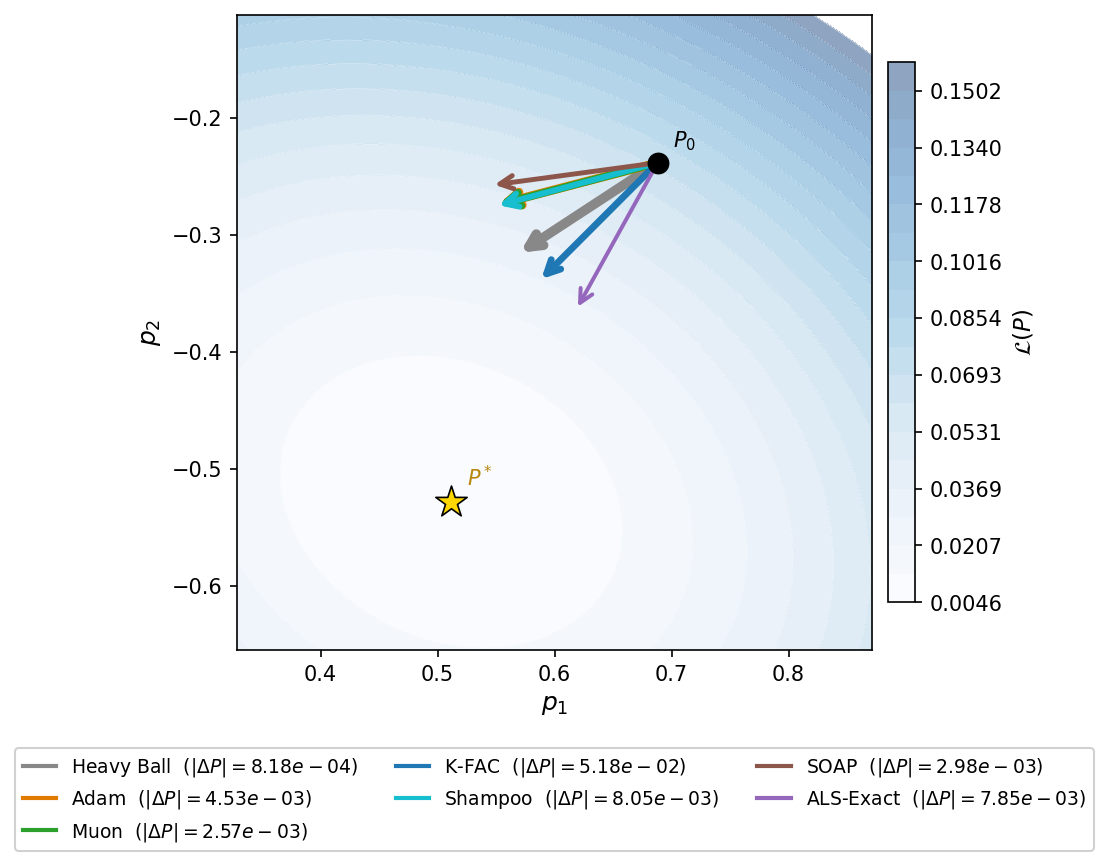
\includegraphics[width=0.6\linewidth]{images/toy_2d_L2_h2.png}
  \caption{One-step update directions in operator space ($L = 2$, $h = 2$,
    Xavier init). Each arrow shows $\Delta P = P_\mathrm{new} - P_0$
    normalized to equal length.}
  \label{fig:2d}
\end{figure}


\subsection{Toy 2D: role of dimensionality and conditioning}
\label{app:exp-machine-precision}

\begin{figure}[h]
  \centering
  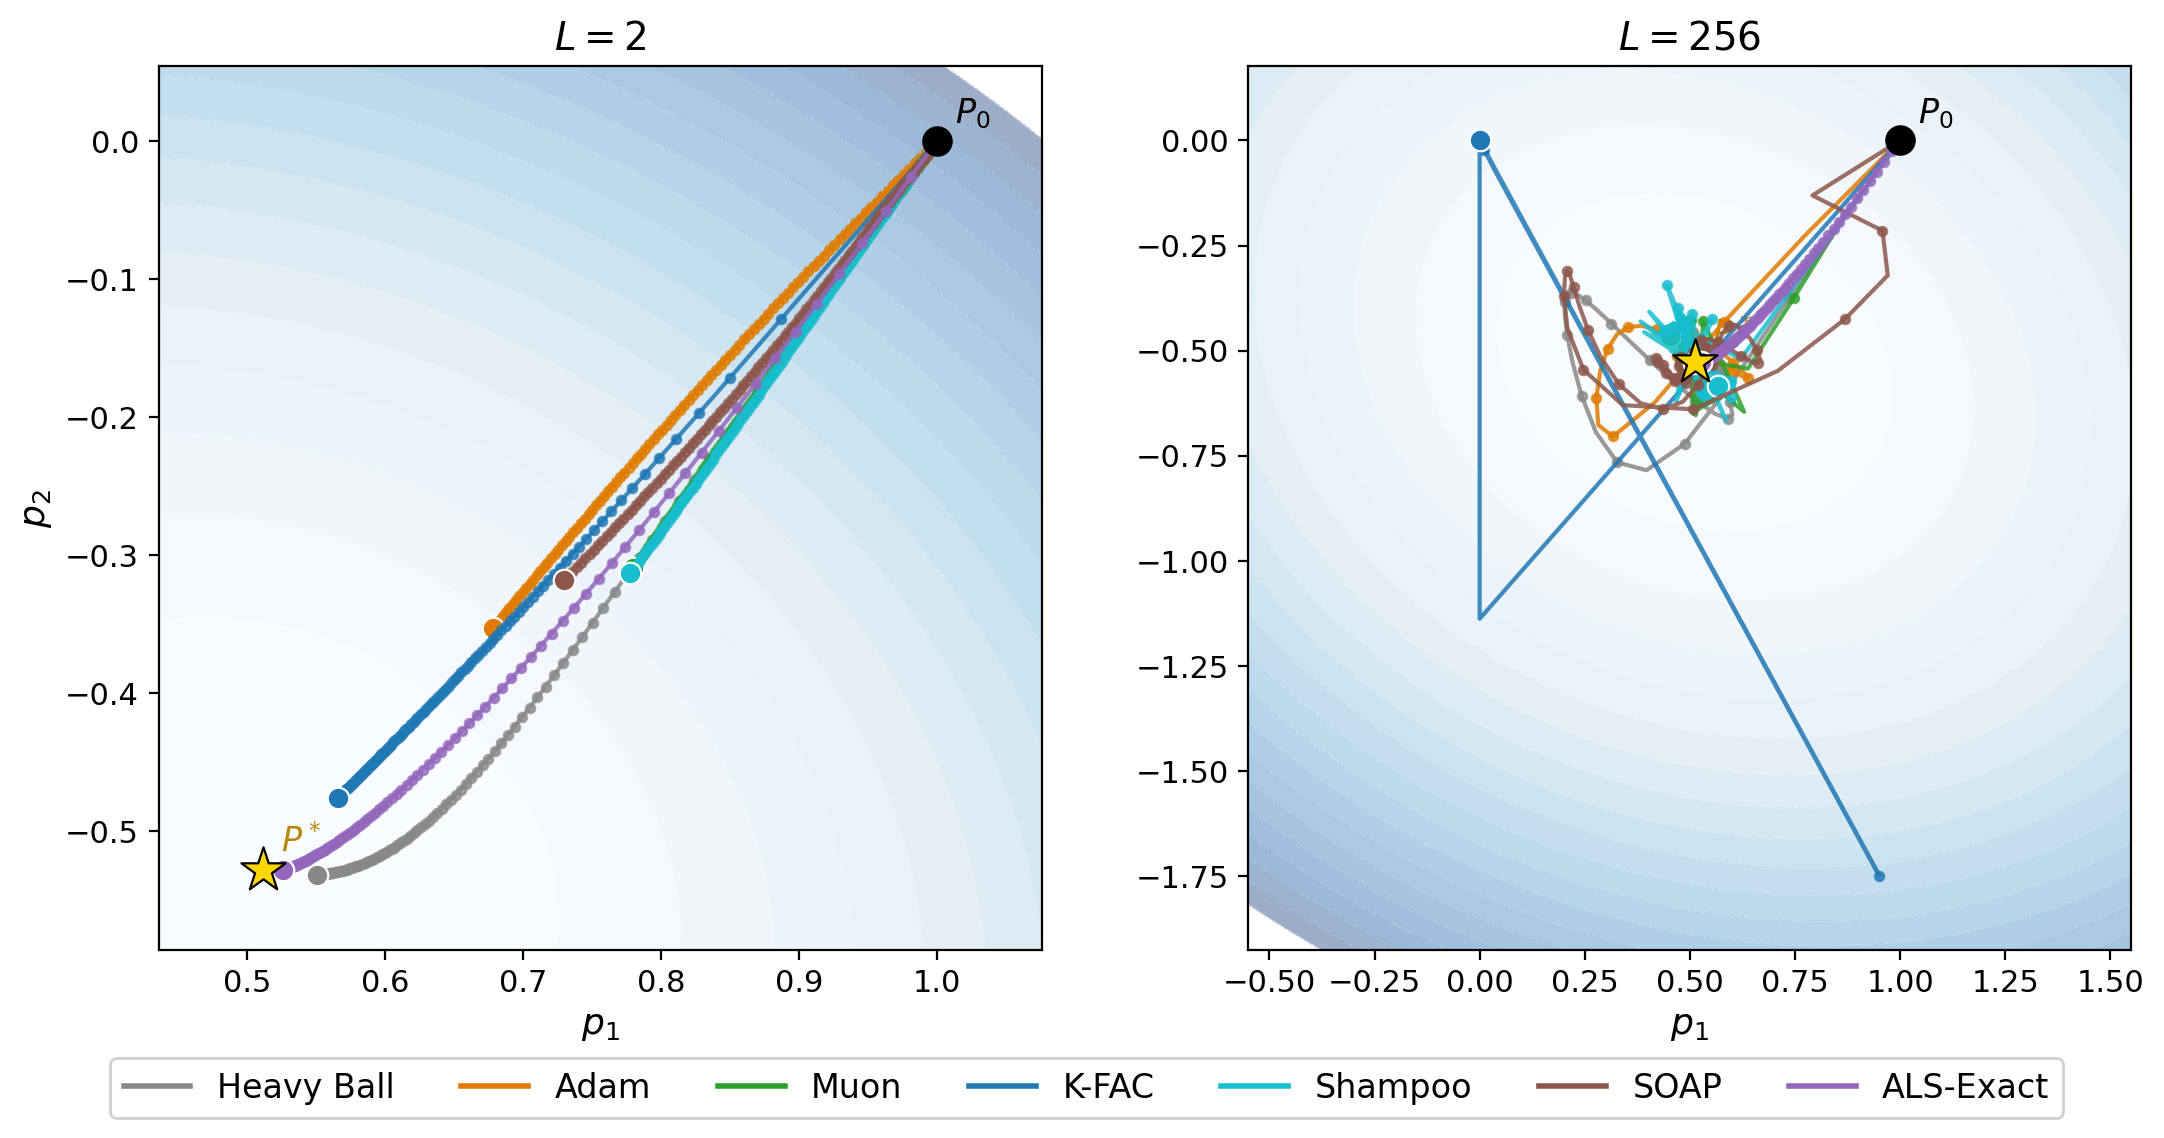
\includegraphics[width=\linewidth]{images/toy_2d_identity_traj_L256.png}
  \caption{Training trajectories in operator space at $L = 256$, $h = 2$,
    identity initialization ($W_k = I$, all context singular values $= 1$).
    All seven optimizers converge to $P^\star$: the combination of perfect
    conditioning and the tiny $d = 2$ operator dimension eliminates the
    gradient-mismatch obstacle.}
  \label{fig:2d-id-traj-L256}
\end{figure}

\begin{figure}[h]
  \centering
  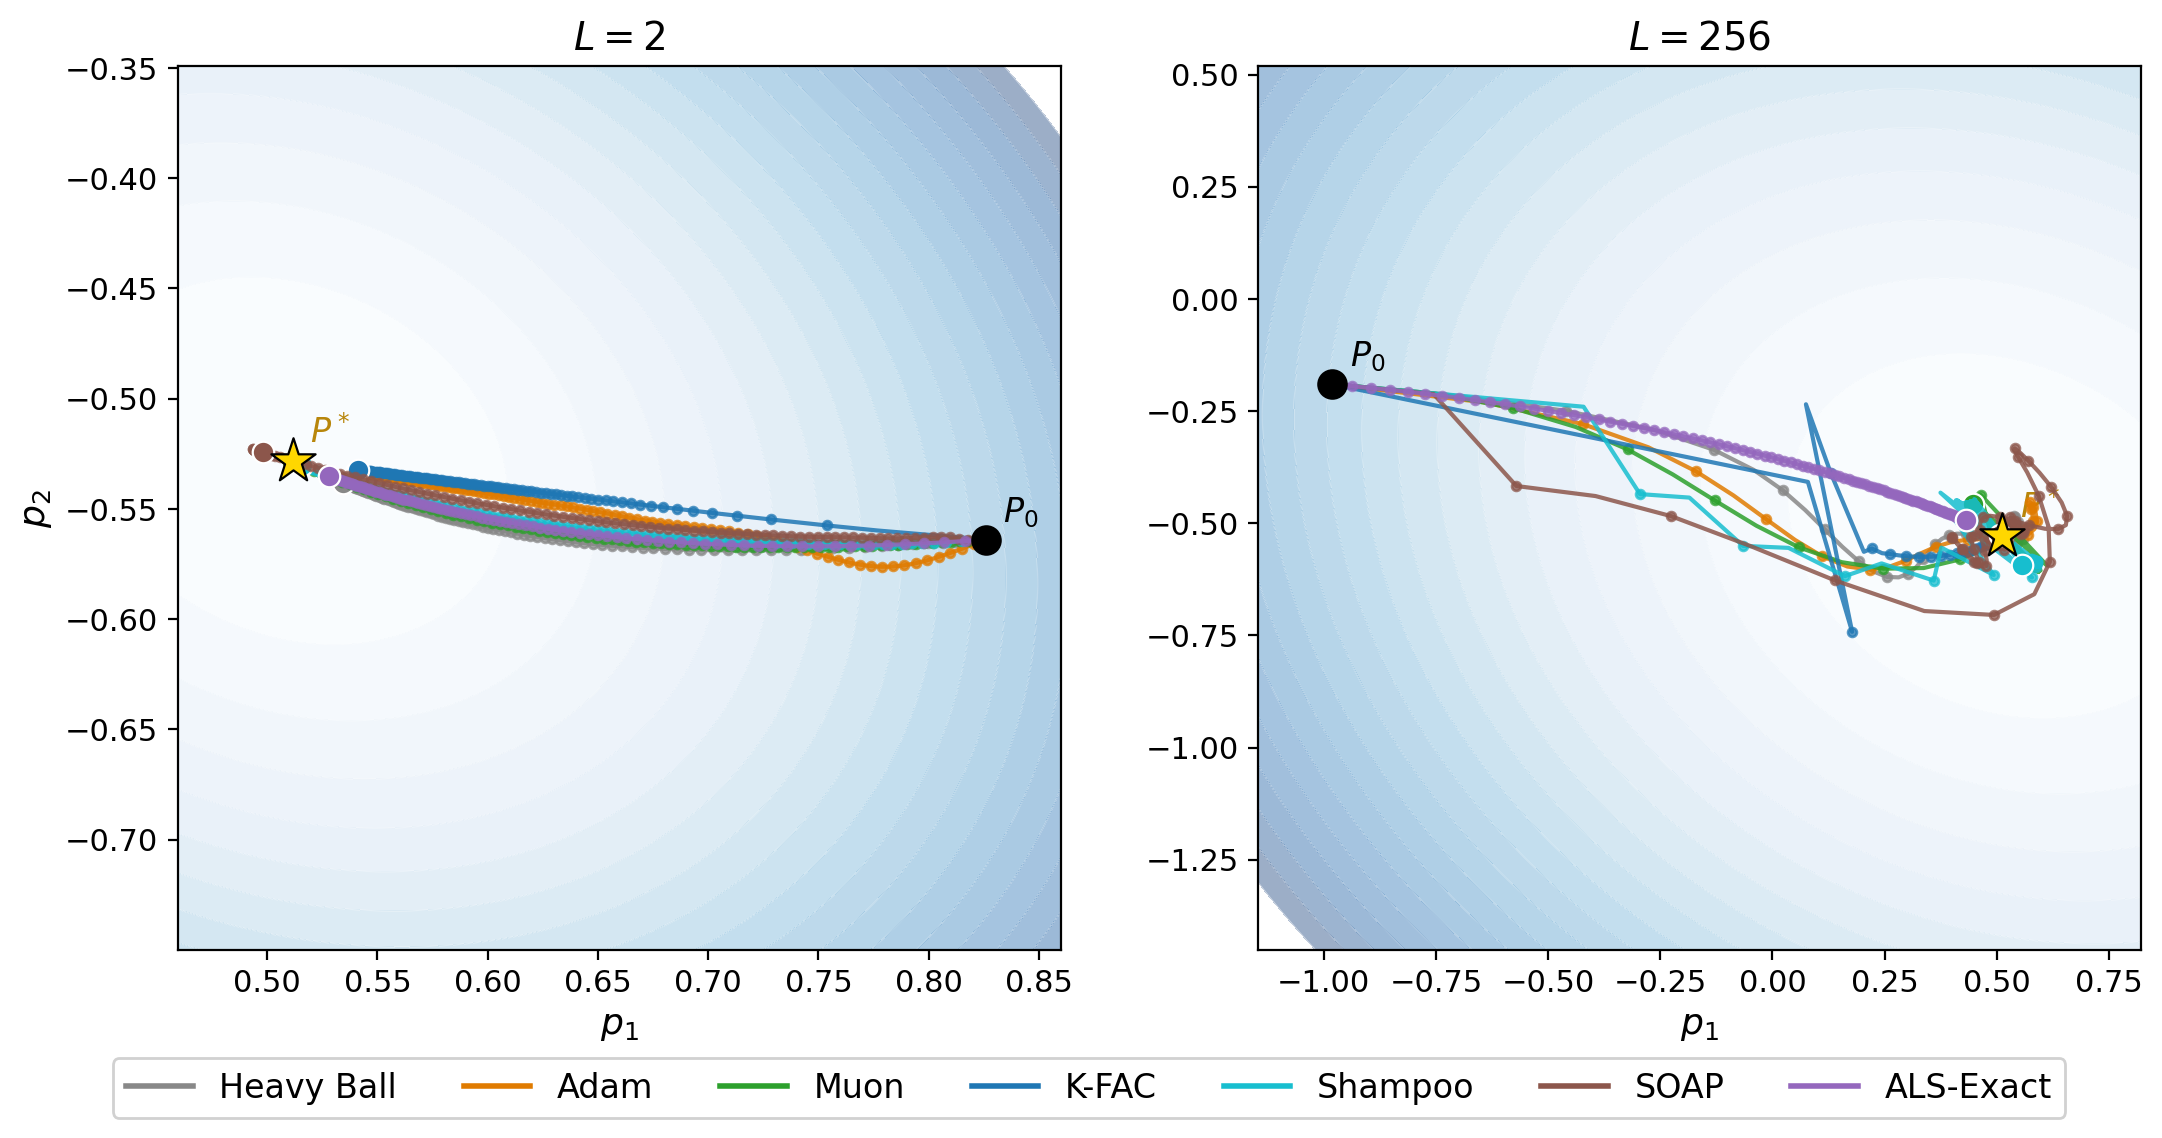
\includegraphics[width=\linewidth]{images/toy_2d_haar_traj_L256.png}
  \caption{Training trajectories at $L = 256$, $h = 2$, Haar (random
    orthogonal) initialization.  All layer singular values remain $1$ but the
    random orientations reintroduce the Gram-matrix anisotropy. We still relatively stable convergence rate for all optimizer, justifying the mismatch appearing in high dimension only. This is expected since there is only 1 well conditioned singular value, the singular "spectrum" is composed of only 1 value and the mismatch doesn't appear.}
  \label{fig:2d-haar-traj-L256}
\end{figure}

The 2D toy ($d = 2$, Section~\ref{sec:exp-2d}) isolates the effect of
initialization conditioning on gradient-based methods.
We repeat the trajectory experiment at $L = 256$ under two initialization schemes.

\paragraph{Identity initialization ($W_k = I$).}
With all layers initialized to the identity every context matrix equals the identity,
all singular values are $1$, and the Gram structure
$\sum_k A_k A_k^\top \otimes B_k^\top B_k = L \cdot I_{d^2}$ is isotropic.
Figure~\ref{fig:2d-id-traj-L256} shows that at $L = 256$ \emph{all seven
  optimizers}, including Heavy Ball, Adam, and Muon, converge to $P^\star$ through a apth close to the best operator updates.
The low operator dimension ($d = 2$) means the effective search space is tiny:
even after accumulating Gram-matrix distortions across 256 layers the residual
mismatch is small enough for coordinate gradient steps to succeed.

\paragraph{Haar (random orthogonal) initialization.}
We next initialize each $W_k$ as an independent Haar-distributed orthogonal matrix
(QR factor of a random Gaussian).  Every layer still has singular values equal to $1$,
so spectral collapse is absent, but the context matrices now have random orientation.
Figure~\ref{fig:2d-haar-traj-L256} shows that at $L = 256$ the gradient-based
optimizers diverge or stall while ALS-Exact continues to converge.
The random orientations reintroduce the Gram-matrix mismatch
$\sum_k A_k A_k^\top \otimes B_k^\top B_k \neq L \cdot I_{d^2}$, which is
sufficient to derail coordinate gradient steps even at $d = 2$.

\paragraph{Interaction of dimension and conditioning.}
Together these two experiments show that \emph{both} low dimensionality
\emph{and} good conditioning are required for coordinate gradient descent to
escape the operator mismatch:
\begin{itemize}
  \item At $d = 2$ with identity init (perfect conditioning), all methods converge
    even at $L = 256$.
  \item At $d = 2$ with Haar init (unit singular values, but random orientation),
    gradient-based methods fail at $L = 256$.
  \item At $d = 16$ with identity init (Section~\ref{sec:exp-deeplinear},
    Figure~\ref{fig:deeplinear-convergence-identity}), gradient-based methods
    stall above $3.5 \times 10^{-1}$ even with perfect conditioning---because the
    increased dimensionality amplifies the Gram-matrix anisotropy.
\end{itemize}
ALS-Exact remains unaffected in all regimes because it solves the operator
sub-problem directly, bypassing the Gram-matrix distortion entirely.


\subsection{FGLN experiments}
\label{app:exp-fgln}

\begin{figure}[h]
  \centering
  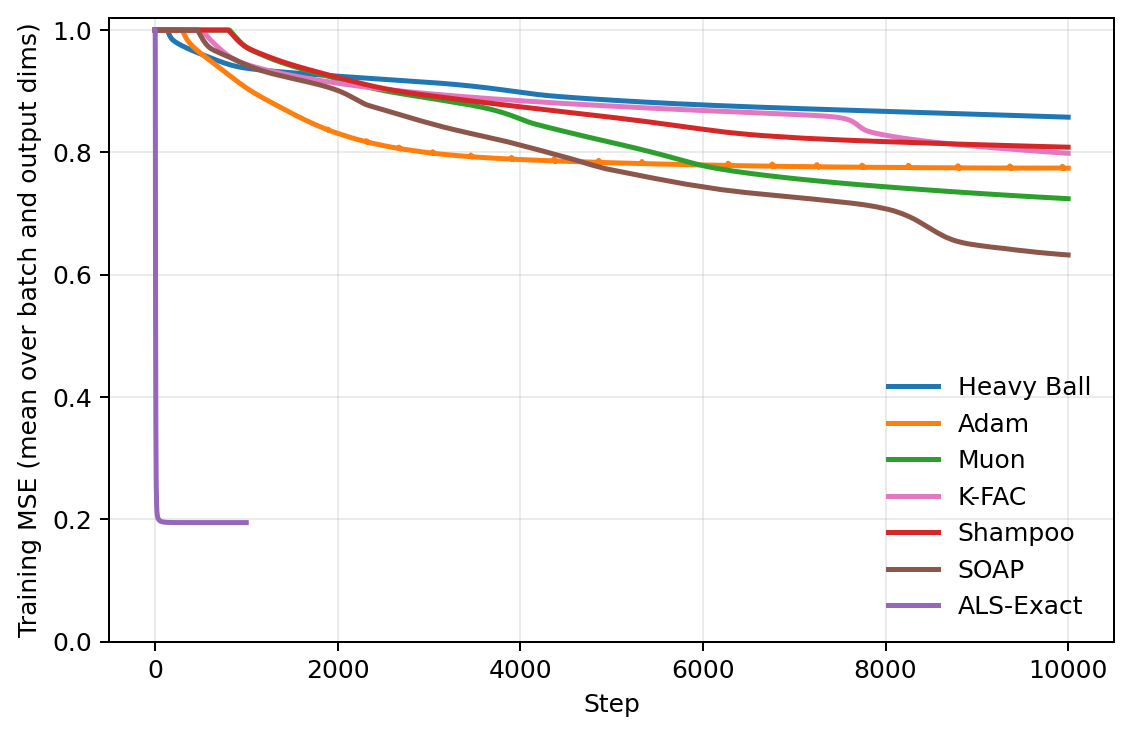
\includegraphics[width=0.6\linewidth]{images/loss_fgln.png}
  \caption{Convergence to $P^\star$ under Xavier initialization ($d = 16$,
    $L = 128$, $N = 64$, isotropic target, up to $10{,}000$ steps) for a FGLN.
    ALS-exact outperforms all gradient based baselines and recovers the isotropic target spectrum up to the rank allowed by the gate pattern. Baselines recover only dominant modes.}
  \label{fig:fgln-convergence}
\end{figure}

\begin{figure}[h]
  \centering
  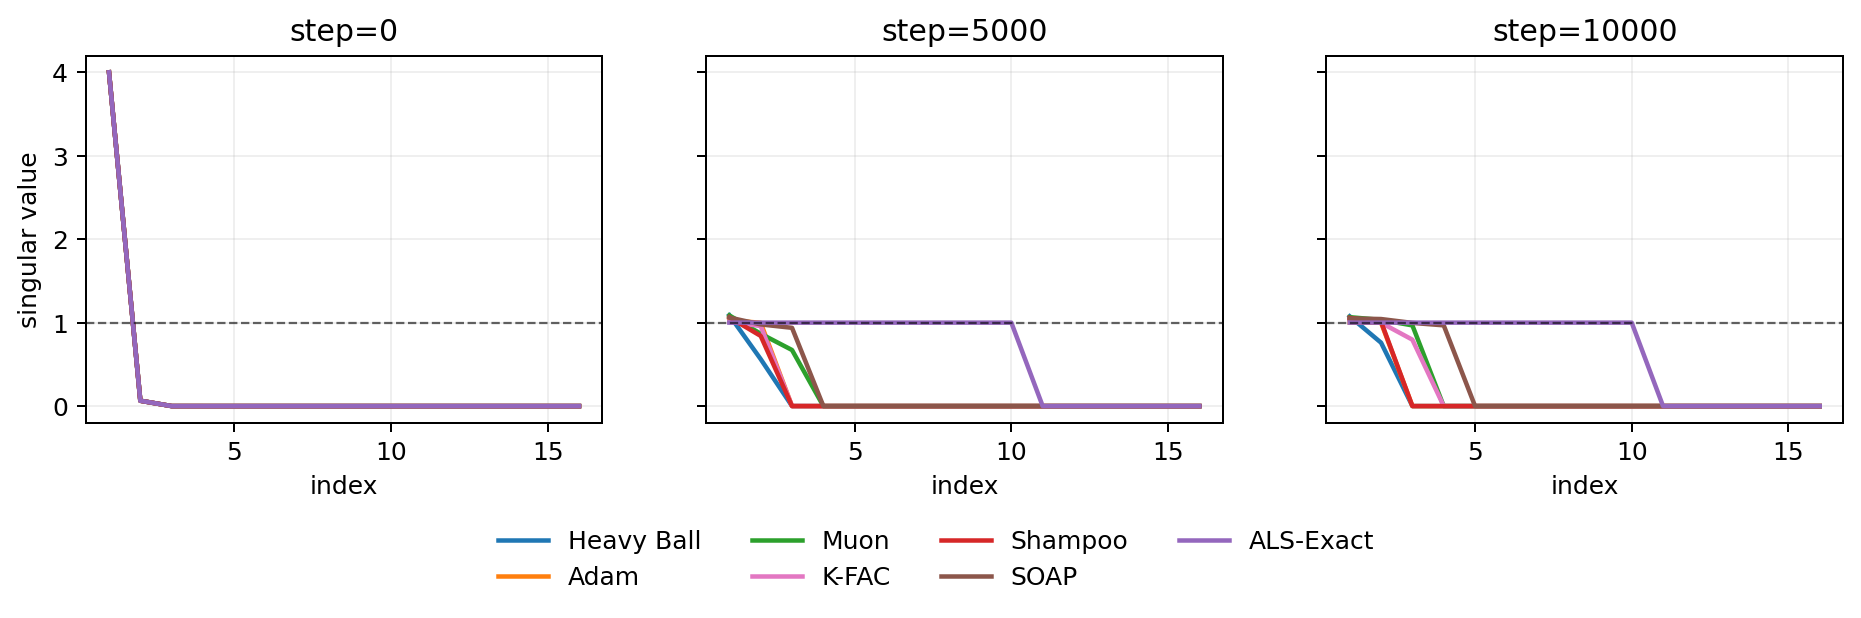
\includegraphics[width=\linewidth]{images/spectrum_fgln.png}
  \caption{Singular-value spectrum of $P(t)$, Xavier initialization ($L = 128$), for a FGLN.
    ALS-exact progressively matches the isotropic target up to the allowed rank by the given gate patterns; baselines remain
    compressed and recover only dominant modes.}
  \label{fig:fgln-spectrum}
\end{figure}


% ==================================================================
%  NEURIPS CHECKLIST  (required, does not count toward page limit)
% ==================================================================
\newpage
\input{checklist.tex}

\end{document}